
\chapter{Literature Review}
\label{ch:chapter2}
As highlighted by section \ref{sec:ch1.section1}, there is a great desire by research scientists for in situ instruments to provide observation data which fills spatial and temporal measurement gaps in Antarctic sea ice monitoring in the Southern Ocean as shown in figure \ref{fig:Antarctica_Southern_Ocean}. This chapter investigates the current use of autonomous monitoring technology used by research scientists in this region focusing on progress made to improving in situ observations and highlighting areas for improvement. 
\begin{figure}[H]
	\centering. 
	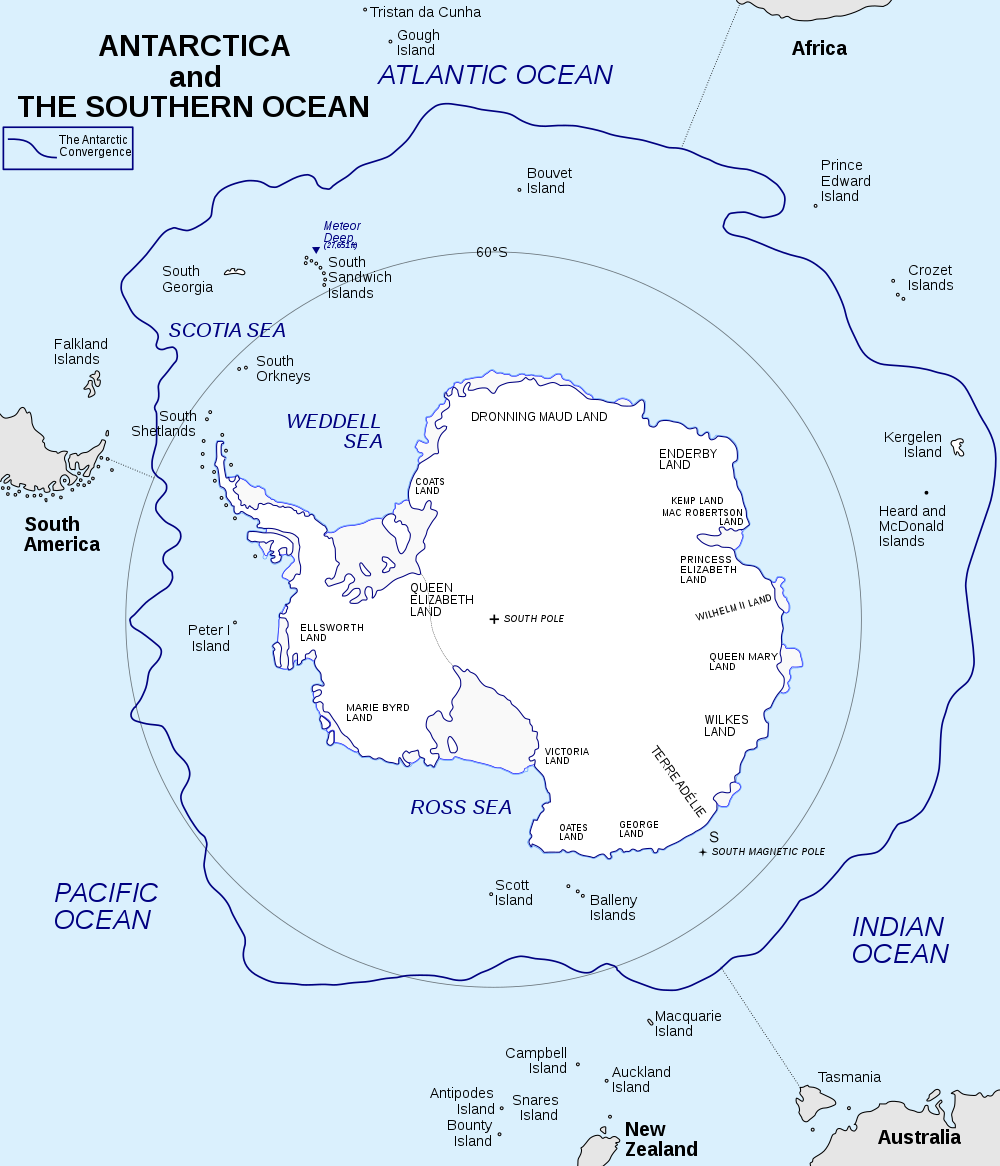
\includegraphics[width = 10cm,height=10cm]{Antarctica_and_the_Southern_Ocean.png}
	\caption{Map of the Southern Ocean surrounding the Antarctic continent. Image created by \textcite{Hogweed2015Ocean} and licensed by CC BY-SA 3.0}
	\label{fig:Antarctica_Southern_Ocean}
\end{figure}

 In this review, a system-level  analysis will be provided where the objectives of each buoy will be discussed in the contexts of the requirements for new technology as highlighted by \textcite{kennicutt2016delivering}.This will include an analysis on how these devices operated in remote conditions and the communication techniques employed in spite of a lack of infrastructure. The system-level analysis will conclude with a discussion of the device measurement objectives, their performance in the Antarctic sea ice region and how this performance compares to their deployment in the Arctic region.\par
 
Next, a subsystem level analysis will be provided discussing how each device met their measurement objectives, what technology was used and how this technology works. Additionally, a comparison of different techniques for each subsystem will be provided among devices with similar components and, where possible, a discussion of their accuracy. This section will also highlight the critical measurement objectives of each device to understand which sub-modules are the most important for remote sensing. Finally, the processing architecture will be discussed in the context of how they were implemented in the devices, what purpose they serve and how the data requirements for each device's sensors were met.
%%%%%%%%%%%%%%%%%%%%%%%%%%%%%%%%%%%%%%%%%%%%%%%%%%%%%%%%%%%%%%%%%%%%%%%%%%%

\newpage
\section{In situ climate sensing technologies}

Autonomous instrumentation has seen increased use for in situ observations in the polar sea ice regions \cite{kennicutt2016delivering}. These devices have typically  been developed by the commercial sector \cite{rabault2017measurements} from companies such as Trident \cite{trident}, MetOcean \cite{uptempo}, Seabird \cite{seabird2021website} and Sea Technology Services (STS) \cite{sts2021website}. Additionally, academic institutions have also developed in situ measurement devices such as The University of Washington's SWIFT buoy \cite{thomson2012wave} or University of Dartmouth's Seasonal Ice Mass Balance (SIMB) buoy \cite{polashenski2011seasonal}. While these technologies have the benefit of reliability, they are often expensive \cite{rabault2017measurements} and inflexible to the specific needs of polar scientists. Technology has reached a point where low-cost and open source alternatives are well documented and reliable enough to be integrated into customized solutions \cite{rabault2019open}.\par 

\begin{figure}[H]
	\centering
	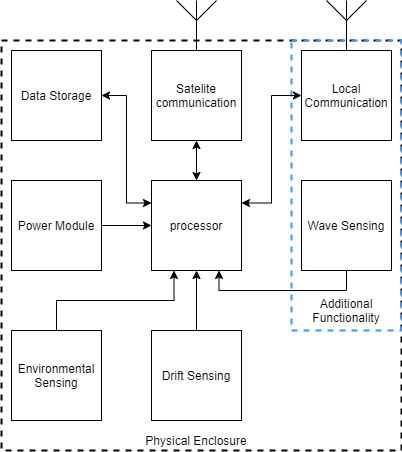
\includegraphics[width = 0.5\linewidth]{device block diagram.png}
	\caption{A block diagram of a typical device for in situ measurements. Each device contains modules for environmental sensing and drift sensing connected to a processor. This can be a micro-controller or microprocessor. Additionally, a data storage module (such as an SD card) is included to store data during the operation. Some device include modules for local communications or wave sensing units. Finally, a remote communication module is included to transfer the data to a research center or a user. The electronics are placed inside a physical enclosure for protection against the polar climate while a portable power module supplies the device during its operation.}
	\label{fig:devblockdiag}
\end{figure}

In this section, a comparison of data collection devices used in the polar regions is presented as well as  description of their design, operation and deployment. Where spossible, certain specifications have been converted into standardized formats. To ensure a fair evaluation, data were collected from the latest technical publication of each platform where possible. These publications may not contain all relevant data. In this case, the data entry has been marked with a "Not reported" or "NR". 


Eight platforms were selected for the comparison and are shown in figure \ref{fig:buoys} with each device designed by a private company or an institution. The key collaborators as well as the name of the institution are provided in table \ref{tab:device_list}. Where a buoy name is not given, the device will be named after the key contributor to the project. These systems have been selected due to their prevalence in global polar/ oceanographic science as well as notability in publications. Device performance will be evaluated in the context of the requirements set out by \textcite{kennicutt2016delivering} for an autonomous in situ measurement device shown in section \ref{sec:ch1.section1}. 

\label{ch2:secdevice}
\begin{figure}[H]
	\centering
	\begin{subfigure}[b]{0.24\textwidth}
		\centering
		\begin{tikzpicture}
			\node[anchor=south west,inner sep=0] (image) at (0,0) { 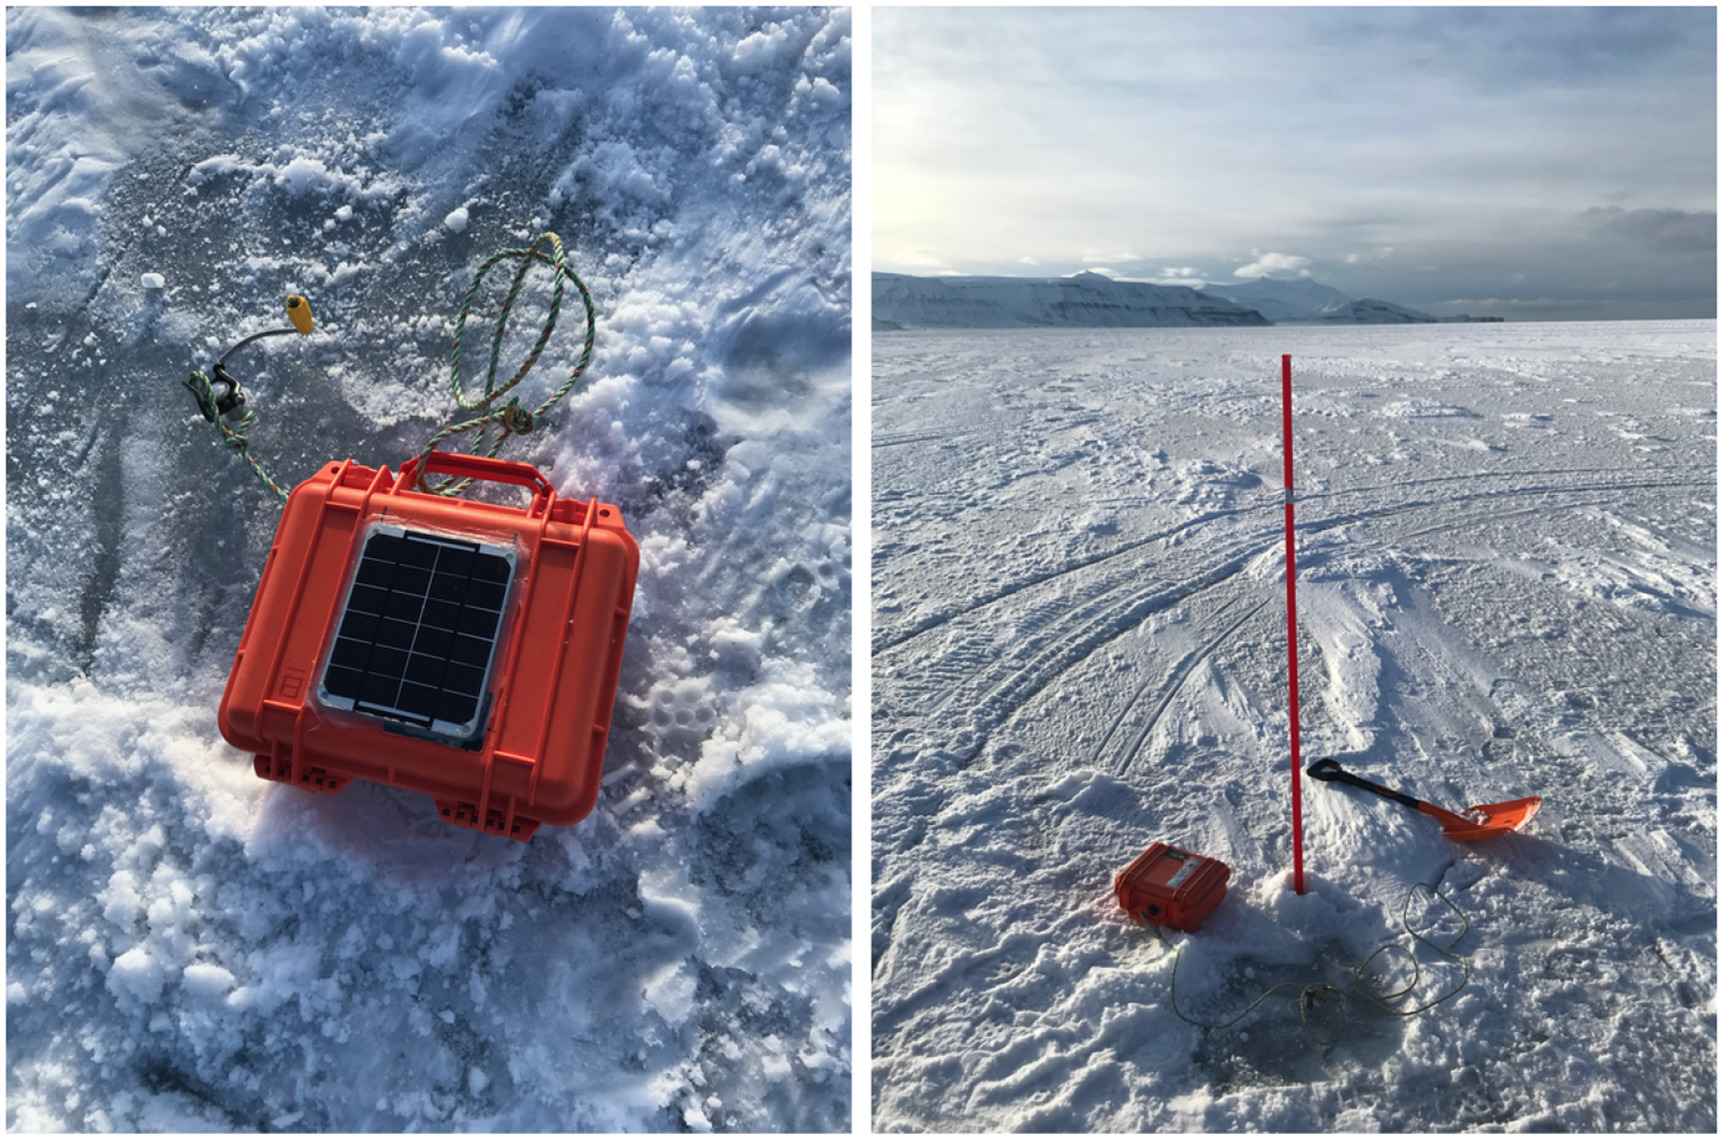
\includegraphics[width = 4cm,height=4cm]{WIIB.jpg}};
			\begin{scope}[x={(image.south east)},y={(image.north west)}]
				\draw[color=black, ultra thin,fill=white] (0.0,0.0) rectangle (0.21,0.16) node[pos=.5] {A};
			\end{scope}
		\end{tikzpicture}
		\label{fig:WIIB}
	\end{subfigure}%
	\hfill
	\begin{subfigure}[b]{0.24\textwidth}
		\centering
		\begin{tikzpicture}
			\node[anchor=south west,inner sep=0] (image) at (0,0) { 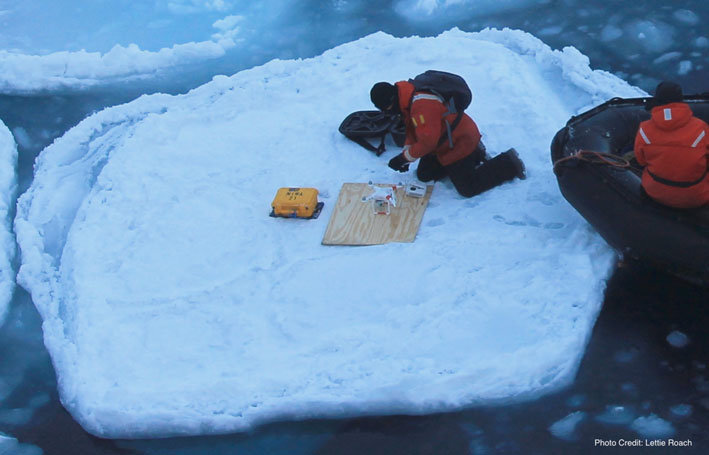
\includegraphics[width = 4cm,height=4cm]{WIIOS.png}};
			\begin{scope}[x={(image.south east)},y={(image.north west)}]
				\draw[color=black, ultra thin,fill=white] (0.0,0.0) rectangle (0.21,0.16) node[pos=.5] {B};
			\end{scope}
		\end{tikzpicture}
		\label{fig:WIIOS}
	\end{subfigure}%
	\hfill
	\begin{subfigure}[b]{0.24\textwidth}
		\centering
		\begin{tikzpicture}
			\node[anchor=south west,inner sep=0] (image) at (0,0) { 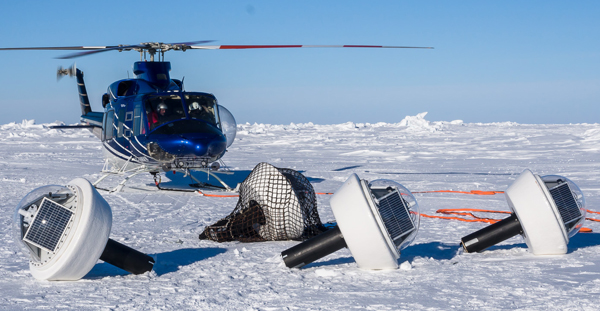
\includegraphics[width = 4cm,height=4cm]{doble.jpg}};
			\begin{scope}[x={(image.south east)},y={(image.north west)}]
				\draw[color=black, ultra thin,fill=white] (0.0,0.0) rectangle (0.21,0.16) node[pos=.5] {C};
			\end{scope}
		\end{tikzpicture}
		\label{fig:NDWB}
	\end{subfigure}%
	\hfill
	\begin{subfigure}[b]{0.24\textwidth}
		\centering
		\begin{tikzpicture}
			\node[anchor=south west,inner sep=0] (image) at (0,0) { 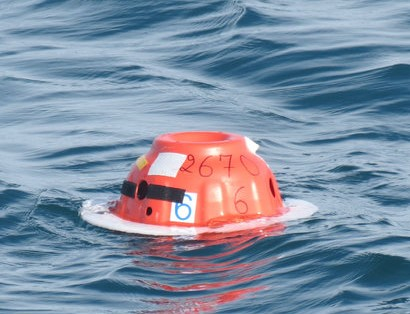
\includegraphics[width = 4cm,height=4cm]{SKIB.png}};
			\begin{scope}[x={(image.south east)},y={(image.north west)}]
				\draw[color=black, ultra thin,fill=white] (0.0,0.0) rectangle (0.21,0.16) node[pos=.5] {D};
			\end{scope}
		\end{tikzpicture}
		\label{fig:SKIB}
	\end{subfigure}%
	\hfill
	\begin{subfigure}[b]{0.24\textwidth}
		\centering
		\begin{tikzpicture}
			\node[anchor=south west,inner sep=0] (image) at (0,0) { 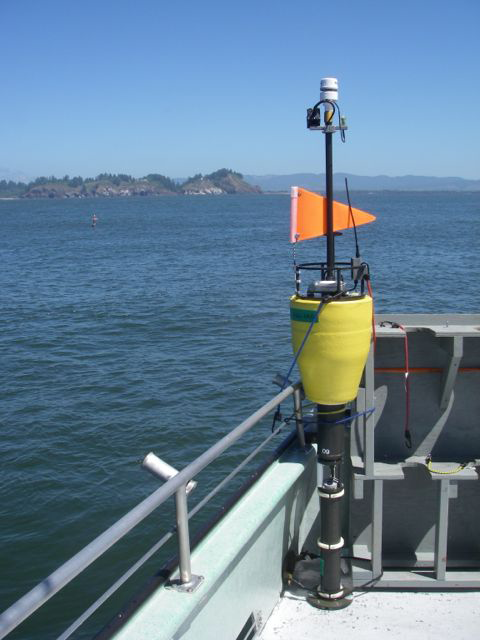
\includegraphics[width = 4cm,height=4cm]{swift_4.png}};
			\begin{scope}[x={(image.south east)},y={(image.north west)}]
				\draw[color=black, ultra thin,fill=white] (0.0,0.0) rectangle (0.21,0.16) node[pos=.5] {E};
			\end{scope}
		\end{tikzpicture}
		\label{fig:SWIFT}
	\end{subfigure}%
	\hfill
	\begin{subfigure}[b]{0.24\textwidth}
		\centering
		\begin{tikzpicture}
			\node[anchor=south west,inner sep=0] (image) at (0,0) { 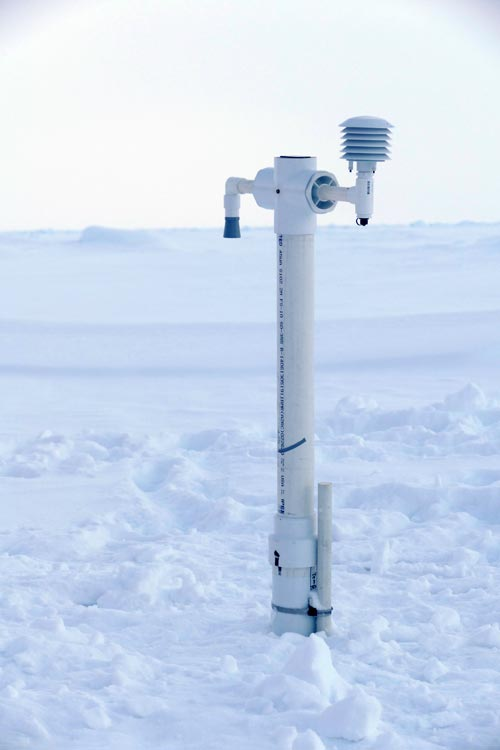
\includegraphics[width = 4cm,height=4cm]{SIMB.jpg}};
			\begin{scope}[x={(image.south east)},y={(image.north west)}]
				\draw[color=black, ultra thin,fill=white] (0.0,0.0) rectangle (0.21,0.16) node[pos=.5] {F};
			\end{scope}
		\end{tikzpicture}
		\label{fig:SIMB}
	\end{subfigure}%
	\hfill
	\begin{subfigure}[b]{0.24\textwidth}
		\centering
		\begin{tikzpicture}
			\node[anchor=south west,inner sep=0] (image) at (0,0) { 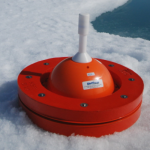
\includegraphics[width = 4cm,height=4cm]{UptempO.png}};
			\begin{scope}[x={(image.south east)},y={(image.north west)}]
				\draw[color=black, ultra thin,fill=white] (0.0,0.0) rectangle (0.21,0.16) node[pos=.5] {G};
			\end{scope}
		\end{tikzpicture}
		\label{fig:UptempO}
	\end{subfigure}%
	\hfill
	\begin{subfigure}[b]{0.24\textwidth}
		\centering
		\begin{tikzpicture}
			\node[anchor=south west,inner sep=0] (image) at (0,0) { 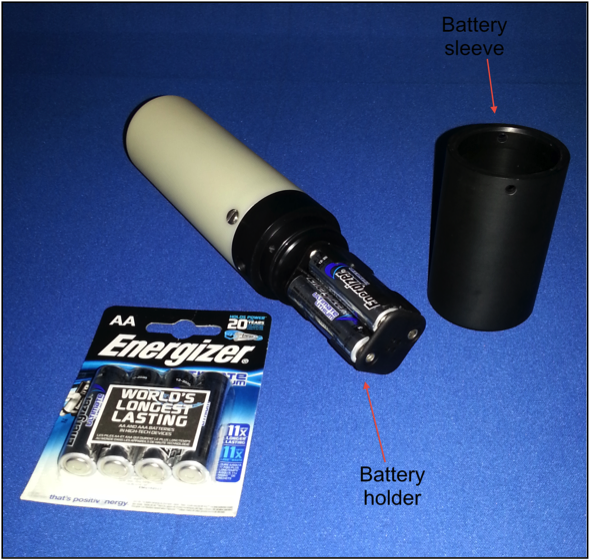
\includegraphics[width = 4cm,height=4cm]{trident.png}};
			\begin{scope}[x={(image.south east)},y={(image.north west)}]
				\draw[color=black, ultra thin,fill=white] (0.0,0.0) rectangle (0.21,0.16) node[pos=.5] {H};
			\end{scope}
		\end{tikzpicture}
		\label{fig:trident}
	\end{subfigure}%
	\hfill
	\caption{ Devices used for the comparison of autonomous instruments deployed in the sea ice region. Each device has been selected for its notability in published work as well as prevalence in sea ice and wave interactions in the Marginal Ice Zones. These devices are: (A) Wave in Ice Buoy developed by \textcite{rabault2017measurements} \cite{rabault2017measurements}, (B) Wave in Ice Observational System by \textcite{kohout2015device} \cite{kohout2015device}, (C) Novel Wave Directional buoys by \textcite{doble2017robust} \cite{doble_wave_2015}, (D) Surface Kinematic buoy by \textcite{guimaraes2018surface} \cite{guimaraes2018surface}, (E) Surface Wave Instrument Float Tracking buoy by \textcite{thomson2012wave}  \cite{jim_swift_2012}, (F) Seasonal Ice Mass Balance buoy by \textcite{polashenski2011seasonal} \cite{simbpic}, (G) Polar ISVP  by MetOcean \cite{uptempo}, (H) Trident buoy by Trident \cite{trident}.}
	\label{fig:buoys}
\end{figure}


A device that has sufficient autonomous and sustained capabilities will operate remotely with no human intervention. Therefore, the operating period of each device will be compared. This is the period between deployment and final transmission where the buoy is active. Additionally, the techniques for remote communication for each buoy will be examined in terms of data rates, coverage and transmission strategy to determine the techniques used to achieve remote communication effectively including a brief overview of available satellite networks. Then, to measure the sensing capabilities of each device, the measurement objectives will be discussed as well as the hardware modules and software used to determine information. To compare the real time data collection, transfer and analysis, the device's processing strategy and storage strategies will be discussed. Data transfer techniques will be analysed with the remote communication section. Finally, device performance in the polar regions will be discussed through the success of each deployment, device deployment time, data integrity will be compared as well as devices that failed and the causes of those failures.

\begin{center}{\setlength{\extrarowheight}{5pt}%
		\begin{longtable}[H]{|>{\RaggedRight}m{0.3\textwidth}|>{\RaggedRight}m{0.2\textwidth}| >{\RaggedRight}m{0.4\textwidth}|}
			\caption{Devices used for the comparison including the device name, lead developer and the institution. These consist of both commercial and institutional devices for in-situ sea ice and wave measurements.}\\
			\hline
			\label{tab:device_list}
			\textbf{Device Name} & \textbf{Developed By} & \textbf{Institution}\\
			\hline
			Waves in Ice Buoy (WIIB) & Jean Rabault & University of Oslo, Norway \cite{rabault2019open} \\
			\hline
			Waves in Ice Observational System (WIIOS) & Alison Kohout & National Institute of Water and Atmospheric Research \cite{kohout2015device}, New Zealand \\
			\hline
			Novel Directional Wave Buoys (NDWB) & Martin J Doble &  Polar Scientific (Ltd.), United Kingdom \cite{doble2017robust}\\
			\hline
			Surface Kinematic Buoy (SKIB) & Pedro Veras Guimarães & Université de Bretagne Occidentale, France \cite{guimaraes2018surface} \\
			\hline
			Surface Wave Instrument Float with Tracking (SWIFT) Buoy & Jim Thompson & University of Washington Applied Physics Laboratory, United States of America \cite{thomson2012wave}\\
			\hline
			Seasonal Ice Mass Balance Buoy (SIMB) & Donald K. Perovich & Dartmouth College \cite{planck2019evolution} \\
			\hline
			Polar ISVP & MetOcean & MetOcean \\
			\hline
			Trident Buoy & Trident Sensor & Trident Sensor \\
			\hline
		\end{longtable}
	}
\end{center}


\section{System Level Overview}

\subsection{Remote Communication}
\label{ch2:sec_remote}

On the Antarctic continent, remote communication is critical for ongoing scientific activities allowing for data to be transmitted from instruments to research stations and camps \cite{Sanghyun2016satellite}. These activities are further supported by high speed, high bandwidth communication networks such as fibre links \cite{jabbar2001multi} however, these networks have been implemented on a small scale to support permanent field camps \cite{Sanghyun2016satellite} on the continent. \textcite{Sanghyun2016satellite} show that communication from polar stations and field sensors to the rest of the world occurs using satellite constellation networks. These constellations are classified as  geostationary earth orbit such as Inmarsat \cite{inmarsat2021website} and Intelsat \cite{intelsat2021website} or low earth orbit (LEO) such as ORBCOMM \cite{orbcomm2021website}, Iridium \cite{iridium2019website}, Globalstar \cite{globalstar2021website} \cite{jabbar2001multi}. GEO satellites consist of 2 - 8 satellites orbiting the equator \cite{jabbar2001multi}. As a result, the network coverage is strong for mid-latitudes and weak for low latitudes. However, these satellites cover large areas providing longer connectivity (of up to 6.5 hours) \cite{Sanghyun2016satellite}. LEO satellites cover less surface area and have a smaller connectivity window (10 - 30 minutes). However, these constellations consist of more satellites. Additionally, the Iridium satellite network is the only LEO network that reaches the polar region \cite{jabbar2001multi} and allow for longer network connectivity. The constellation consists of 66 satellites \cite{Sanghyun2016satellite} and is well optimised for marine applications making it suitable for Southern Ocean sea ice applications. Iridium is a satellite network with global coverage and a variety of modems for various IoT uses. The company offers four main data services. Each service places constraints on the data transmission rates, bandwidth and modem selection. Each modem runs a data service that dictates the transmission rates, bandwidth and protocols.  Table \ref{tab:iridium service} shows the available network services. Furthermore, a full description of these modems is shown in table \ref{tab:ir_devices}. \par 

\begin{figure}[H]
	\centering
	\begin{subfigure}[b]{0.3\textwidth}
		\begin{tikzpicture}
			\node[anchor=south west,inner sep=0] (image) at (0,0) { 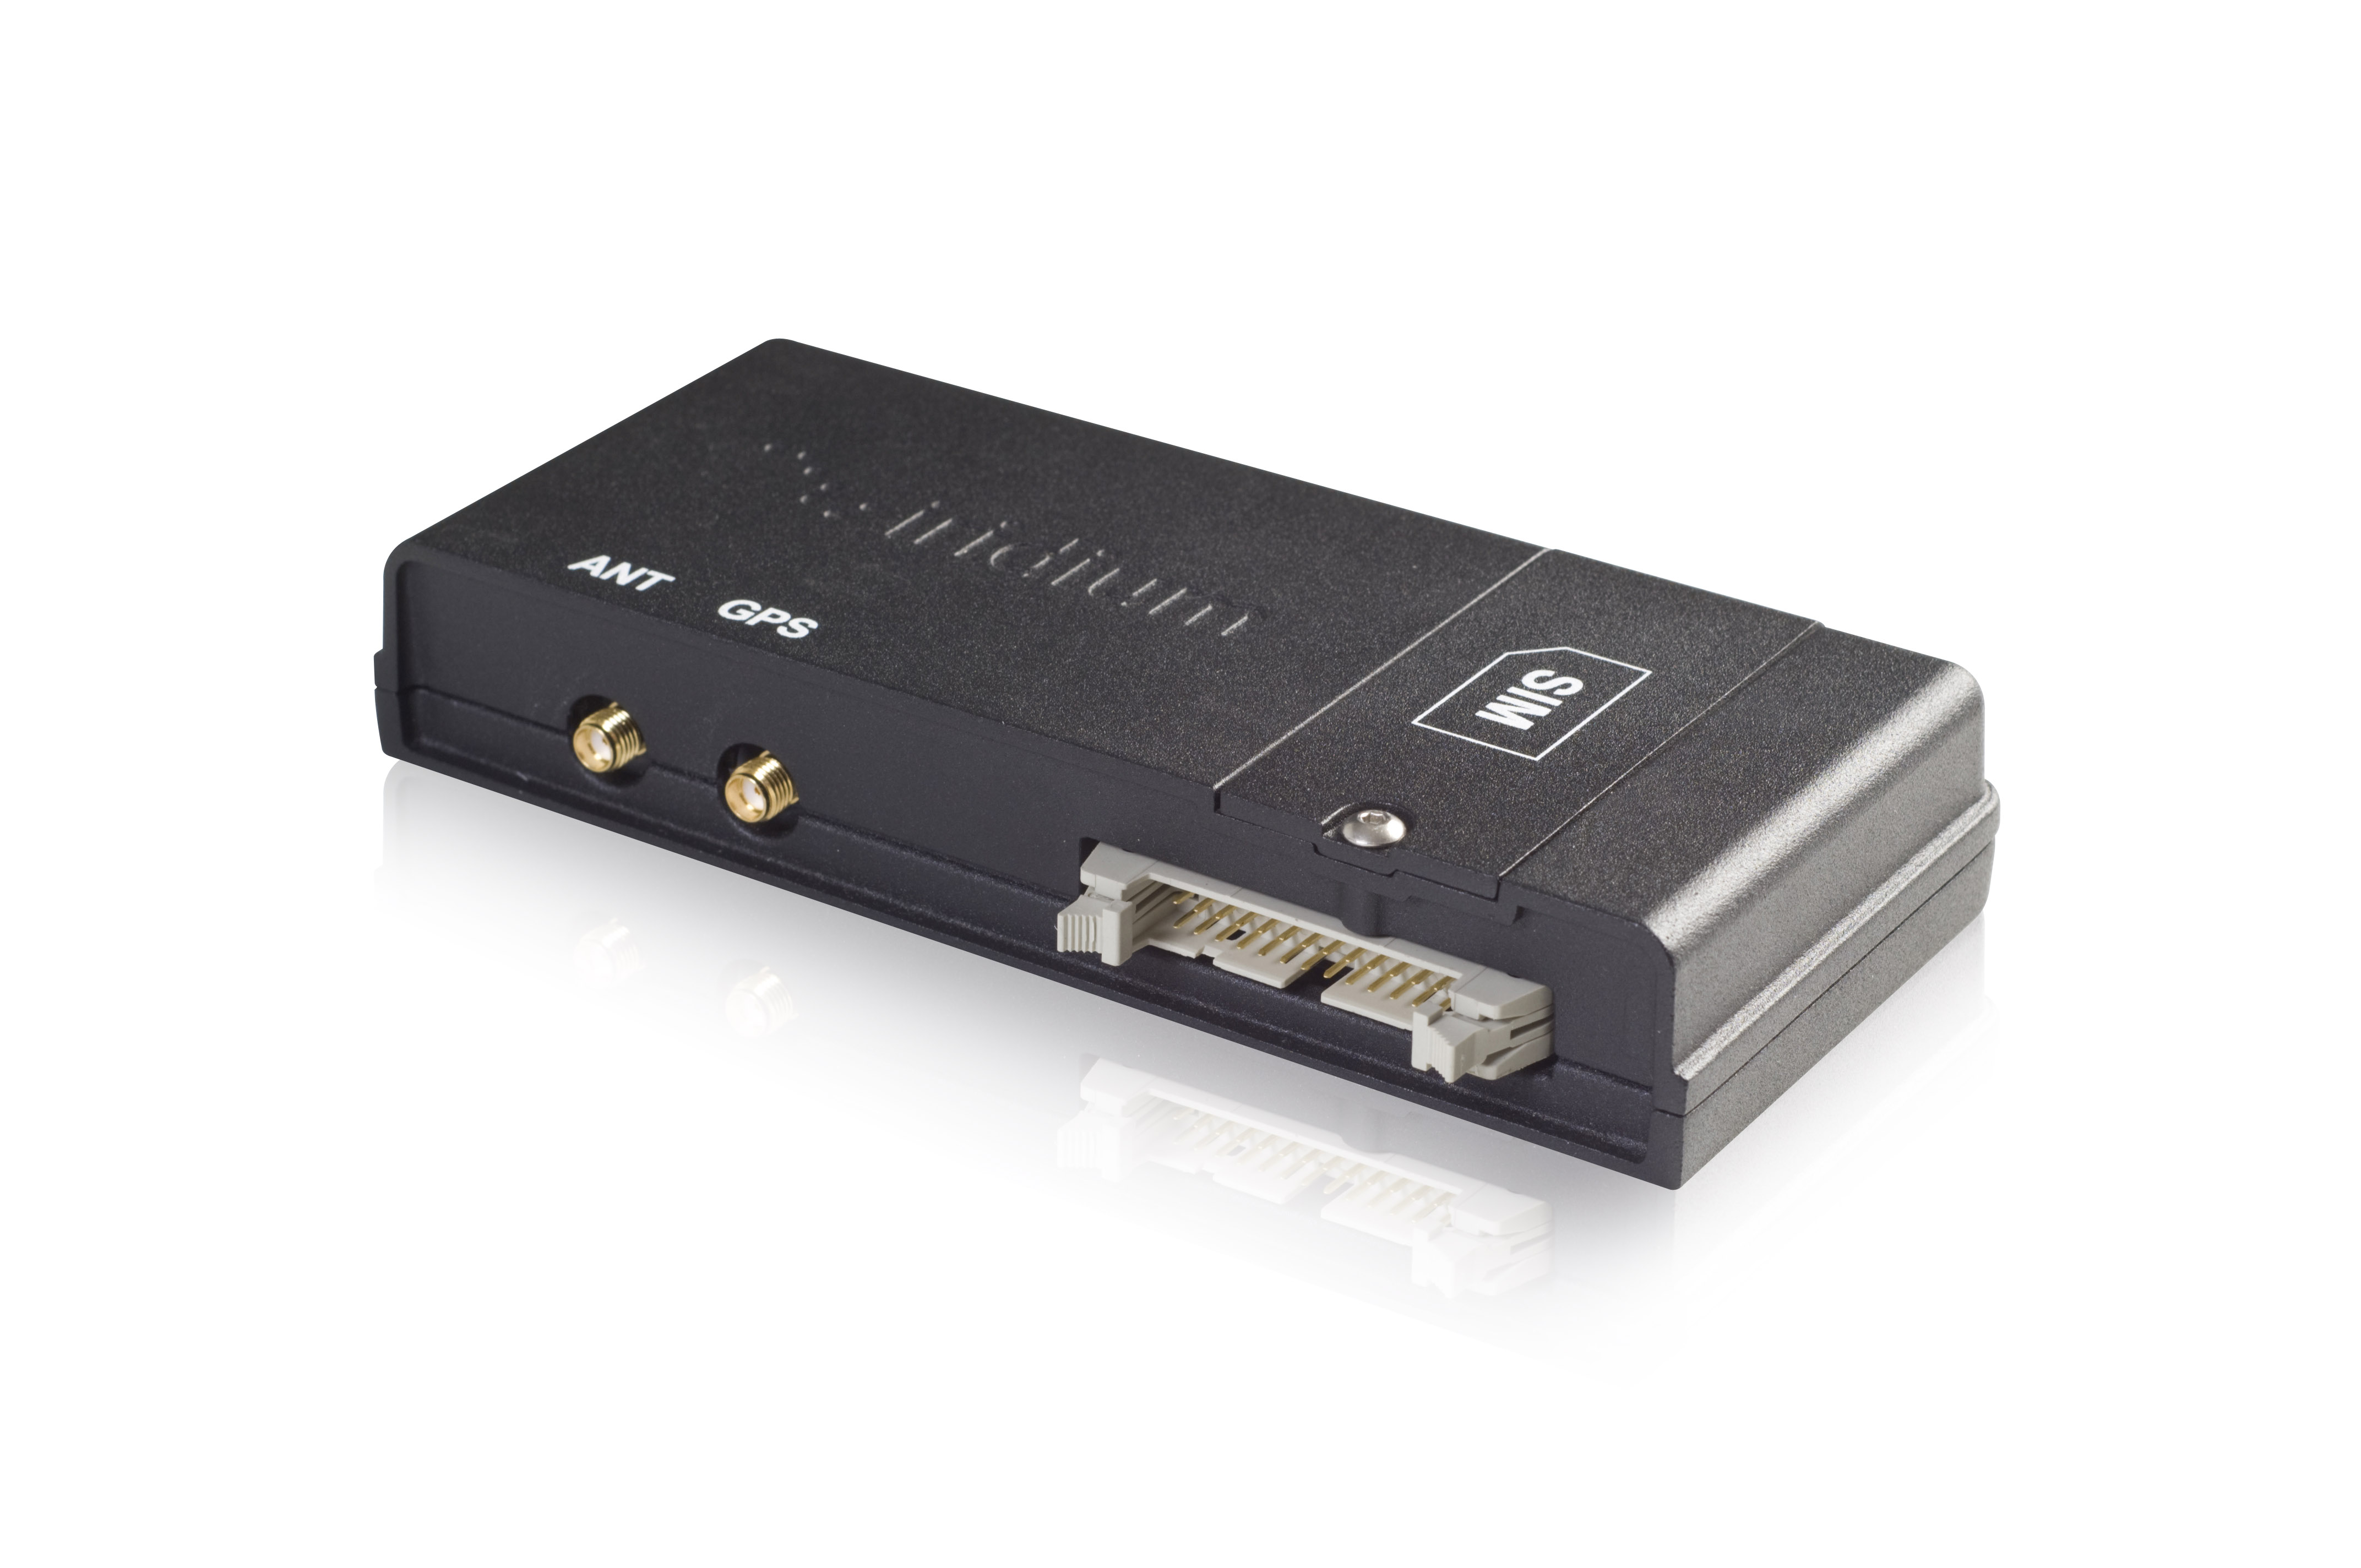
\includegraphics[width = 3cm,height=3cm]{9522B.png}};
			\begin{scope}[x={(image.south east)},y={(image.north west)}]
				\draw[color=black, ultra thin,fill=white] (0.0,0.0) rectangle (0.21,0.16) node[pos=.5] {A};
			\end{scope}
		\end{tikzpicture}
	\end{subfigure}%
	\hfill
	\begin{subfigure}[b]{0.3\textwidth}
		\begin{tikzpicture}
			\node[anchor=south west,inner sep=0] (image) at (0,0) { 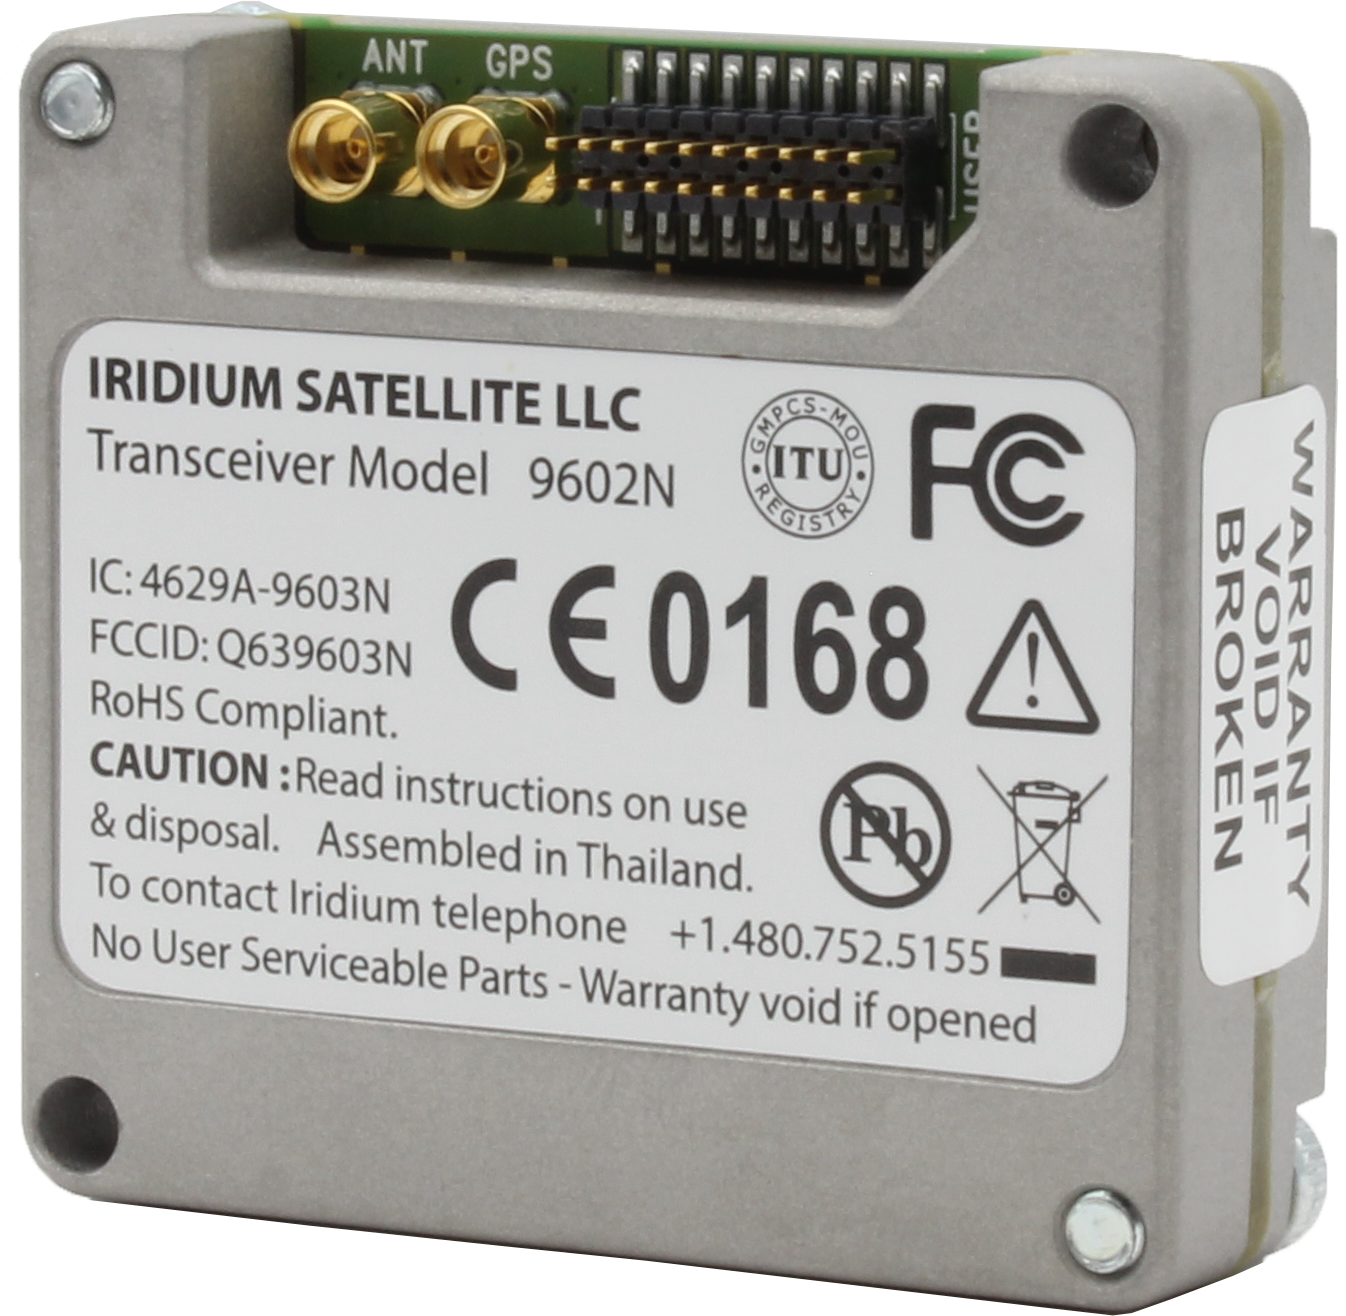
\includegraphics[width = 3cm,height=3cm]{9602.png}};
			\begin{scope}[x={(image.south east)},y={(image.north west)}]
				\draw[color=black, ultra thin,fill=white] (0.0,0.0) rectangle (0.21,0.16) node[pos=.5] {B};
			\end{scope}
		\end{tikzpicture}
	\end{subfigure}%
	\hfill
	\begin{subfigure}[b]{0.3\textwidth}
		\begin{tikzpicture}
			\node[anchor=south west,inner sep=0] (image) at (0,0) { 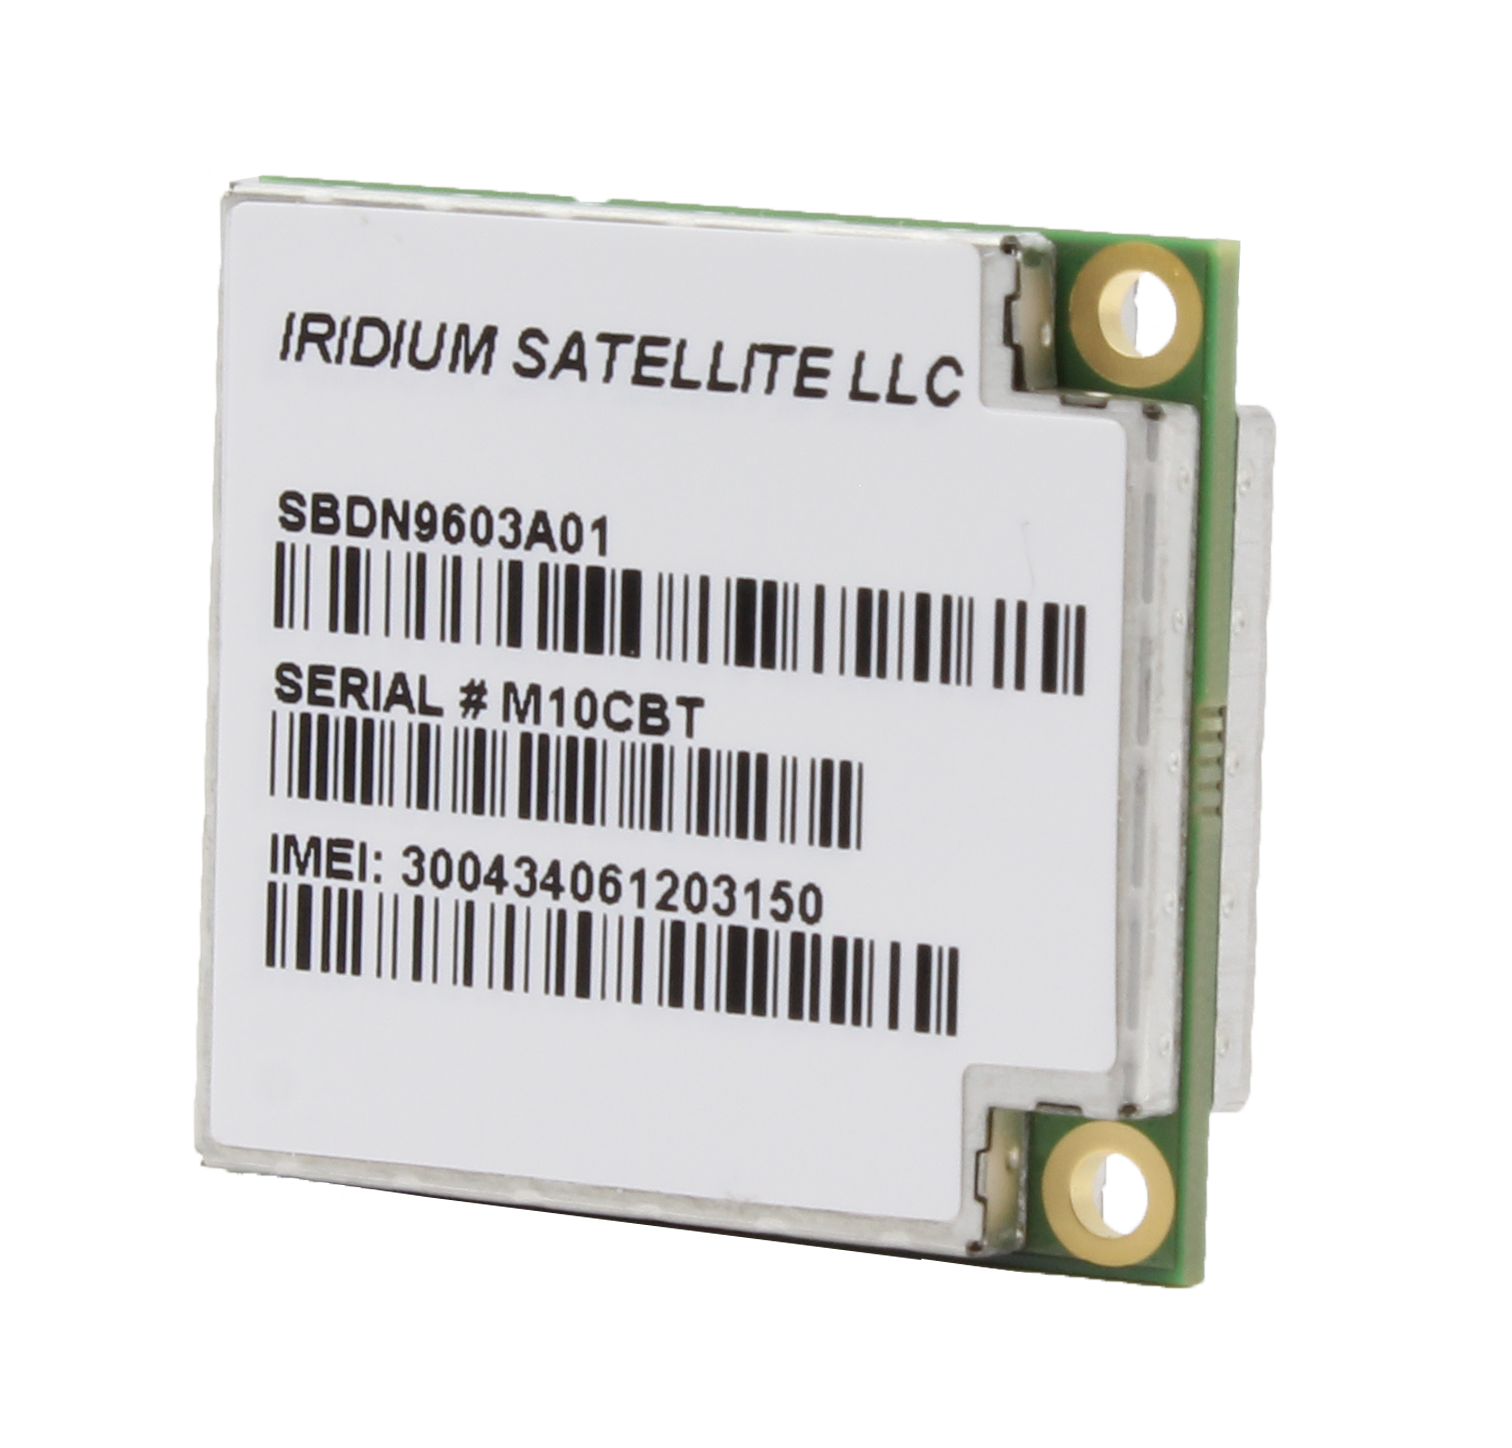
\includegraphics[width = 3cm,height=3cm]{9603.png}};
			\begin{scope}[x={(image.south east)},y={(image.north west)}]
				\draw[color=black, ultra thin,fill=white] (0.0,0.0) rectangle (0.21,0.16) node[pos=.5] {C};
			\end{scope}
		\end{tikzpicture}
	\end{subfigure}%
	\hfill
	\caption{Examples of popular iridium modems selected for remote communications. The 9522B modem (A) (image source: \cite{9522B}), 9602 modem (B) (image source: \cite{9602}) and 9603 modem (C) (image source: \cite{9603})} 
	\label{fig:irid_modem}
\end{figure}

Table \ref{tab:device_transmissionstrategies} shows the satelite network used by each device. All device use Iridium as the primary remote communication method. Other short range wireless systems such as Zigbee \cite{guimaraes2018surface} are alluded to however these systems are only used when the device is close by. Notably, The SIMB buoy details consideration for remote communication using the ARGOS satellite network however, the unreliability of the network resulted in irregular timestamped data \cite{planck2019evolution}. The network service, modem and transmission strategy of each device is shown in table \ref{tab:device_transmissionstrategies}.


\begin{table}[H]
	\centering
	\caption{ The following Iridium modems are compared in their key specifications. devices in the table were suitable for IoT applications based on prevalence in literature and recommendations from the manufacturer. Key parameters include weight, power consumption and transmission latency.Taken from \cite{iridium_product} }
	\label{tab:ir_devices}
	\resizebox{\textwidth}{!}{%
		\begin{tabular}{|l|c|c|c|c|c|}
			\hline
			\textbf{Device Name: } & \textbf{9602} & \textbf{9603} & \textbf{9522B\footnotemark} & \textbf{9523} & \textbf{Edge}\\
			\hline
			Weight (g) & 30 & 11.4 & 420 & 32 & 330 \\
			\hline
			Input Voltage (VDC) & 5 &5 & 4 -32 & 3.2-6 & 9 - 32V\\
			\hline
			Idle Current (mA) & 35 & 34 & 250 & 70 &300\\
			\hline
			Transmit Current (mA)& 140 & 145 &2.5$\times10^3$&500& 300 \\
			\hline
			Recieve Current (mA) & 40 & 39 &2.5$\times10^3$&110 & 300 \\
			\hline
			Packet Latency (s) &  20  &  20 & N/A &45 s& 20s\\
			\hline
			Price &	R2,526.07\footnotemark & 2,526.07\footnotemark & R23,317.40\footnotemark& R13,123.10\footnotemark & R5,638.18\footnotemark\\
			\hline
	\end{tabular}}
\end{table}
\footnotetext[2]{source: \url{https://www.rock7.com/shop-product-detail?productId=49}}
\footnotetext[3]{source: \url{https://www.rock7.com/shop-product-detail?productId=50}}
\footnotetext[4]{source: \url{https://satellitephonestore.com/catalog/sale/details/iridium-9522b-transceiver-496}}
\footnotetext[5]{source: \url{https://www.africasatellite.com/Iridium-9523-Core-Module-p/iridium-9523-core-module.htm}}
\footnotetext[6]{source: \url{https://www.rock7.com/shop-product-detail?productId=56}}

%figure of open-source buoy using the modem
Unanimously, all devices use the Iridium satellite network for remote communication with the Iridium 9602/3 SBD modem being used the most.  This choice is justified for its small form factor, low power and easy interfacing as shown in table \ref{tab:ir_devices} however it suffers greatly from limited bandwidth having a maximum transmission size of 340 bytes. Systems that use these modems for transmission of wave data rely on complex data processing algorithms and therefore do not transmit the raw time series. The only notable exception to this is the wave buoy developed by \textcite{doble2017robust} which continuously transmitted  data from an attitude and heading reference system (AHRS) as well as IMU time series data once every minute. For this purpose, they used the 9522B modem which allowed for continuous transmission using the RUDICS data service. This modem, along with the SBD modem used for the SWIFT Buoy also has a much larger SBD data buffer (1.92KB) However this device draws the most current during idle, transmit and receive states. Additionly this modem is expensive costing R23,317.40 compared to the 9523 (R13,123.10) and the 9602/3 (R2,526.07).  

\subsection{Power Supply}

A robust power supply is critical to support the functionality of a remotely deployed device. A successful power supply can extend the deployment range, duration, processing capabilities and functionality of sensors \cite{kennicutt2016delivering}. Device operation in the Southern Ocean MIZ presents a challenge where the constant freezing/ refreezing of the ocean surface layer prevents long-term infrastructure from being implemented. Hence, a remote device for sea ice monitoring requires a portable power source. Figure \ref{fig:powermoddiag} shows a diagram of a typical power module for a remote sensing device.

\begin{figure}[H]
	\centering
	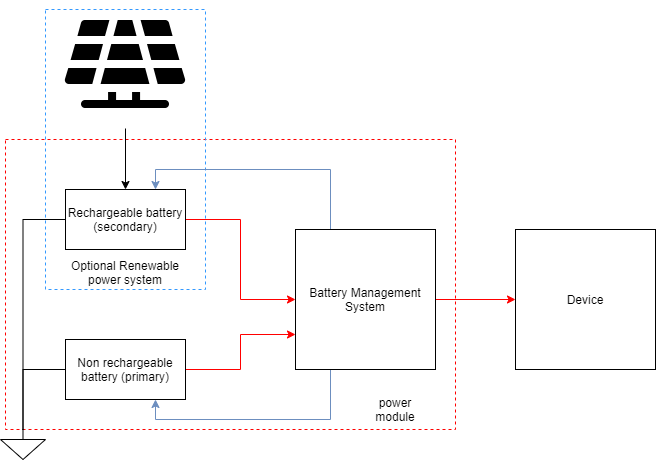
\includegraphics[width = \linewidth]{power module diagram.png}
	\caption{A block diagram of a typical power module for a remote sensing device based off the information from \cite{rabault2019open,doble2017robust,vidal2019xev}. Batteries are used as a primary source of energy which is connected to a battery management system to control and regulate the power supply to the device. optionally, solar panels are implemented with a rechargeable battery as a secondary power supply. Shown in the figure: flow of power (red), control lines (blue) and ground (black).}
	\label{fig:powermoddiag}
\end{figure}

Batteries such as lithium-ion are commonly used as sources of power for in situ devices. Batteries typically fall into one of two categories:
\begin{enumerate}
	\item Primary: Cells that cannot be recharged once they are depleted. These batteries have a high energy density and can store charge for long periods.\cite{besenhard2008handbook}
	\item Secondary: Cells that can be recharged. These cells are more cost effective with longer usage cycles \cite{besenhard2008handbook}.
\end{enumerate}

Lithium  Ion and Alkaline batteries are examples of primary cells that have commonly been used as they provide a cost effective solution due to their high energy density and long-term consistent life cycles \cite{zareer2018review}.  Secondary cells such as lead-acid, nickel-metal hydride and lithium polymer are commonly used coupled with a secondary charging circuit such as a solar panel \cite{manimekalai2013overview} to provide a more constant source of power. While batteries are cost effective solutions, the climate of the Southern ocean can affect the battery performance. Freezing air temperatures can reduce the capacity of a standard lithium cell by up to 50\% for temperatures below $-10^\circ C$ \cite{doble2017robust,ZHANG2003137}. Additionally, frozen batteries/ ice formation on batteries can stop them from working \cite{doble2017robust,manimekalai2013overview}. A solution to compensate for this reduction is to use rechargeable batteries coupled with a renewable power sources such as solar \cite{doble2017robust,rabault2019open}, wind and geothermal energy \cite{manimekalai2013overview}. Solar photovotaic (PV) cells is the fastest growing renewable energy source with the highest energy density \cite{jordehi2016parameter}. PVs have numerous advantages such as low maintenance and operational costs, wide temperature operations and long life-cycles \cite{jordehi2016parameter} which makes them ideal for long term operation in remote environments. However, the power output of PV cells are significantly affected by weather conditions \cite{sharma2015solar}. Therefore, areas with poor sunlight coverage will not benefit from solar panels.Therefore this energy source is not suitable for winter Antarctic expeditions due to the lack of sunlight \cite{lever2006solar}. Additionally, power generation from solar panels is inconsistent and requires an additional storage bank capable of frequent charging and discharging. Wind energy can provide a viable alternative to solar energy. \textcite{vichi2019effects} show that the Southern Ocean hosts strong, consistent winds. However, the design and implementations have not been discussed in any of the literature. Therefore this options is provided as an area for future research. Finally, a critical component of the power system is a battery management system. This allows the power supply to operate under safe conditions while meeting performance requirements \cite{vidal2019xev}. This module includes power monitoring, power control and energy cycle optimization. Table \ref{tab:device_power_source} below shows the power sources used by each device and the strategy used to manage it.
\begin{table}[H]
	\centering
	
	\caption{A comparison of power supply strategies of the different devices  showing the the power source, topology of the power supply module as well as the voltage supplied at the output of the module. Information that was unavailable at the time of research has been labeled as "Not reported"}
	\label{tab:device_power_source}
	
	\setlength{\extrarowheight}{5pt}%
	\resizebox{\textwidth}{!}{%
		\begin{tabular}{|>{\centering}m{3cm}|>{\raggedright\arraybackslash}m{4cm}|>{\raggedright\arraybackslash}m{4cm}|>{\raggedright\arraybackslash}m{4cm}|>{\raggedright\arraybackslash}m{4cm}|>{\centering\arraybackslash}m{3cm}|}
			\hline
			\textbf{Device Name} & \textbf{Primary Power Source} & \textbf{Secondary Power Source} & \textbf{Battery Management System} & \textbf{Output Regulation Strategy} & \textbf{Output Voltage} \\
			\hline
			WIIB & Lithium Iron Phosphate (LiFePO4) battery & None & ATMega328P for Power control & Boost Converter & 5V \\
			\hline
			WIIOS & Alkaline battery & None & Integrated into firmware & 8-cell series configuration, no regulator & 12V \\
			\hline
			NDWB & Alkaline battery & Solar panel and lead-acid battery & Not Reported & Not Reported & 12V \\
			\hline
			SKIB & Lithium thionyl chloride (LiSOCl2) battery & None & Not Reported & Not Reported & 3.6V \\
			\hline
			SWIFT & Alkaline or Lithium  battery& None & Not Reported & Not Reported & 14V \\
			\hline
			SIMB & Alkaline battery & None & Not Reported & LMZ12003 Step Down Converter (5V, 3.3V)\par MIC29201-12W Low dropout regulator (12V) & 3.3V \par 5V \par 12V\\
			\hline
			Polar ISVP & LiSOCl2 battery & None & Not Reported & Not Reported & 12V \\
			\hline
			Trident & Lithium cell battery & None & integrated into firmware & Low dropout regulator & 5V\\
			\hline
	\end{tabular}}
\end{table}
\footnotetext{Information available online at \url{https://github.com/jerabaul29/LoggerWavesInIce_InSituWithIridium/blob/master/ElectronicsList/list.md}}

Table \ref{tab:device_power_source} shows the power supply strategies of each device. All systems use primary batteries as a source of power with the most common choice being alkaline or lithium-based batteries. However, \textcite{doble2017robust} is the only exception where a secondary power source was added consisting of a solar panel and lead-acid batteries. As a consequence of the added power system the NDWB had an increased weight which affected its portability and ease of handling. This will be discussed further in subsection \ref{subsec:sec2_overallcost}. Furthermore, systems deployed in the Arctic Marginal Ice Zone have been designed with a recharging system such as a solar panel in the case of WII Buoy and NDWB, however, most long-range deployment buoys have opted for non-rechargeable systems composed of lithium thionyl chloride (LISOCL2) or alkaline batteries. In the case of the high-power buoys (SIMB, WIIOS, NDWB, Polar ISVP) an array of 3.3V -3.7V cells is connected to provide a nominal voltage in series with a regulator to provide a stable output. The strategy for each system is to pack as many batteries in as possible to satisfy the long-term energy requirements \cite{doble2017robust,rabault2019open}. Finally, few devices have reported their battery management strategies. \textcite{rabault2019open} used an ATMega328P microcontroller as a power controller for their device which monitored the status of the battery. \textcite{trident} and \textcite{kohout2015device} however integrated power control into their main firmware allowing for them to control and monitor their power source off a single processor.

\subsection{Polar Performance}

This section outlines the deployment of the systems in the Arctic/Antarctic marginal ice zones and compares the survivability and performance of each system. The focus of this section will be predominantly on devices deployed in the marginal ice zone. Table \ref{tab:device_deployment} shows the significant deployment locations in the Arctic and Antarctic sea ice zones as well as the deployment objectives of each device. 

\begin{table}[H]
	\centering
	\caption{ comparison between the functionality and purpose of the buoy showing the critical measurements as well as the significant deployment locations either in the polar ice zones or in a location critical to the validation of the device.}
	\label{tab:device_deployment}
	\setlength{\extrarowheight}{5pt}
	\resizebox{\textwidth}{!}{
		\begin{tabular}{|l| >{\raggedright\arraybackslash}m{5cm}|>{\raggedright\arraybackslash}m{5.4cm}|>{\raggedright\arraybackslash}m{5cm}|}
			\hline
			\textbf{Device name} & \textbf{Deployment objectives} & \textbf{Antarctic Deployments} & \textbf{Arctic deployments}\\
			\hline
			\multirow{3}{*}{WIIB} & Wave energy attenuation &  Ross Sea landfast ice \cite{rabault2020development} &  Templefjord (Svalbard) landfast ice \cite{rabault2019open} \\
			& Significant wave height &  & Northeast Barents sea \cite{rabault2019open}\\
			& Data quality && \\
			\hline
			\multirow{5}{5cm}{WIIOS} &Ice drift&Ross sea marginal ice zone \cite{kohout_smith_roach_williams_montiel_williams_2020}&\multirow{5}{*}{-}\\ 
			& Waves in ice & Ross Sea packed ice zone \cite{kohout2015device} & \\ 
			& Ambient temperature & Weddel Sea marginal ice zone \cite{vichi2019effects,albarello2020drift}& \\
			& Atmospheric pressure && \\
			\hline
			\multirow{4}{*}{NDWB} & Ice drift  & \multirow{4}{*}{ - } & \multirow{4}{5cm}{Beaufort sea \cite{doble2017robust}} \\
			& Wave induced ice breaking &&\\
			& Ambient temperature &&\\
			& Atmospheric pressure &&\\
			\hline
			\multirow{2}{*}{SKIB} & Ice drift &\multirow{2}{*}{-} & North Atlantic ocean (France) \cite{guimaraes2018surface}\\
			& Surface waves &&\\
			\hline
			\multirow{6}{*}{SWIFT} & Surface images & Ross Sea \cite{ackley_2020_seaice} & Chukchi sea \cite{hosekova2020Attenuation} \\
			& Ocean waves & Weddel sea \cite{DeSanti2018OceanWave} &  Beaufort sea \cite{lund2018Arctic} \\
			& Turbulence profiles &&\\
			& Ocean current profiles &&\\
			& Conductivity && \\
			&Wind speed and direction && \\
			\hline
			\multirow{6}{*}{SIMB} & Surface and bottom ice position &Weddel sea \cite{hoppmann2015fmot} & Beaufort sea marginal ice zone \cite{PLANCK2019102792} \\
			& Snow depth& & \\
			& Atmospheric pressure&& \\
			& Ambient temperature &&\\
			& Vertical temperature profile& & \\
			& GPS Location&&\\
			\hline
			\multirow{3}{*}{Polar ISVP} & Sea ice drift & \multirow{3}{5.4cm}{Weddel Sea marginal ice zone \cite{deVos2021evaluating,grosfeld2016online,ipab}} & \multirow{3}{5cm}{Western Arctic Ocean \cite{lei2020comparisons}}\\
			& Ambient temperature & &\\
			& Atmospheric pressure &&\\
			\hline
			\multirow{3}{*}{Trident} & Sea ice drift & \multirow{3}{5.4cm}{Weddel sea \cite{vichi2019effects,alberello2019drift}}
			& \multirow{3}{*}{-}\\
			& Ambient temperature & &\\
			& Battery voltage &&\\
			\hline
		\end{tabular}
	}
\end{table}

\textcite{kohout2015device} deployed five Wave in Ice Observational Systems (WIIOS) in the East Antarctic marginal ice zone during the Sea Ice Physics and Ecosystem Experiment (SIPEX) mission\footnote{1st deployment occured September 2012 \cite{kohout2015device}} with the goal of capturing wave in ice events with measurement goals shown in table \ref{tab:device_deployment}. Three devices were deployed by helicopters on ice floes while two devices were deployed via the ships crane. \textcite{kohout2015device}
note that deployment via crane was successful in spite of 7 m swell and 25 $m \text{ }s^{-1}$ winds. The device was fitted inside a Pelican box with a sealed membrane surrounded by a tyre for protection and flotation in case of melting \cite{kohout2015device}. Consequently, this places the buoy directly on the surface of the floe rendering it susceptible to snow build up and flooding as mentioned in the previous sections.  After deployment, the crew received 600 samples of data over 39 days in total. However, the first device failed 20 hours after deployment coinciding with the first large wave event captured the buoys \cite{kohout2015device}. The second large wave event resulted in the failure of two more systems just 9 days after deployment \cite{kohout2015device}. The fourth buoy lasted for 17.5 days. The final buoy survived the longest at 39 days. As a result only one device lasted for the expected time with the majority of data captured during calm events.

\begin{figure}[H]
	\centering
	\begin{subfigure}[b]{0.45\textwidth}
		\begin{tikzpicture}
			\node[anchor=south west,inner sep=0] (image) at (0,0) {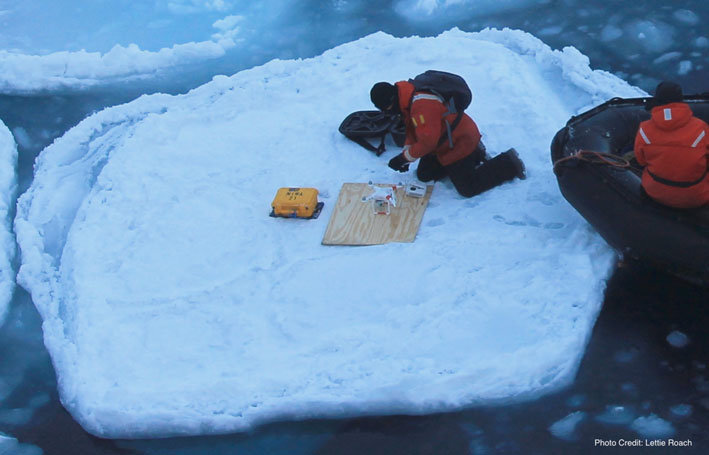
\includegraphics[width = 6cm,height=8cm]{WIIOS.png}};
			\begin{scope}[x={(image.south east)},y={(image.north west)}]
				\draw[color=black, ultra thin,fill=white] (0.0,0.0) rectangle (0.21,0.16) node[pos=.5] {A};
			\end{scope}
		\end{tikzpicture}
	\end{subfigure}%
	\hfill
	\begin{subfigure}[b]{0.45\textwidth}
		\begin{tikzpicture}
			\node[anchor=south west,inner sep=0] (image) at (0,0) { \includegraphics[width = 6cm,height=8cm]{Basket.jpg}};
			\begin{scope}[x={(image.south east)},y={(image.north west)}]
				\draw[color=black, ultra thin,fill=white] (0.0,0.0) rectangle (0.21,0.16) node[pos=.5] {B};
			\end{scope}
		\end{tikzpicture}    
	\end{subfigure}
	\caption{ Examples of different deployment protocols for ice tethered devices. In regions of consildated ice in favourable conditions, manned crews will step foot on the ice to deploy the device (A) (image source: \cite{kohout2020observation}), in unfavourable conditions, devices may deployed from a basket attached to a crane (B). A manned crew will lower the buoy on a suitable ice floe from the safety of the basket (image source: N. Taylor) }
	\label{fig:deploy}
\end{figure}
Two additional WIIOS buoys were deployed by NYU Abu Dhabi \textcite{vichi2019effects,alberello2019drift} during the winter\footnote{first deployment occured in July 2017 \cite{vichi2019effects,alberello2019drift}}. Here, the buoys lasted significantly shorter than the previous deployment. The first system survived for 8 days while the second system survived for 3 weeks in spite of measures taken to place the device in power saving mode \cite{vichi2019effects,alberello2019drift}. This was achieved by lowering the sample period from to 2 hours. Consequently, the lower temporal resolution resulted in a significantly reduced accuracy of the ice deformation calculations \cite{vichi2019effects,alberello2019drift}. However, despite this low resolution, by operating at a temporal scale of 3 hours or less \cite{vichi2019effects,alberello2019drift}, one can effectively and accurately capture ice drift speed as well as the oscillations surrounding the movement. Additionally, \textcite{vichi2019effects,albarello2020drift} discuss the deployment of two Wave in Ice Observation Systems similar to the ones by \cite{kohout2015device}. 2 devices were deployed on two separate ice floes 3 m in diameter and 100 km  the ice edge \cite{vichi2019effects,albarello2020drift}. One system survived for 8 days and 18 hours while sampling every 15 minutes before transmission ended \cite{vichi2019effects,albarello2020drift}. The second buoy however, survived for 6 days sampling every 15 minutes until it switched to power saving mode surviving for a total time frame of 3 weeks. \textcite{vichi2019effects,alberello2019drift} deployed a second pair of WIIOS buoys however, the first buoy stopped responding after 3 days while the second buoy survived for only 16 days \cite{vichi2019effects}. While the buoys survival is largely attributed to power optimisation, the lifespan could be influenced by the selection of the ice floe. Ice floe size and proximity to the ice edge affect the exposure of the floe to open-ocean processes and storms \cite{vichi2019effects}. This could result in failure due to ice mechanics which is discussed in section \ref{ch2:sec3_failiure}. \par 

\textcite{rabault2019open} deployed the waves in ice buoy (WIIB) WIIB on land-fast ice in the Ross sea \cite{rabault2020development} to test the device's performance in the Antarctic. In a similar fashion to the WIIOS buoy, the device was placed in a pelican case and attached to a flotation device, however, expected survival time for this device was significantly lower compared to the WIIOS devices: a maximum of 8 days \cite{rabault2019open} of continuous operation. The buoys by \textcite{kohout2015device} were designed to be expendable whereas the buoys by \textcite{rabault2019open} were designed to be retrievable. Additionally, the WIIB devices were deployed in the summer\footnote{First deployment date: December 2019 \cite{rabault2019open}}. Two devices were deployed in proximity however an ice break event resulted in the separation of the devices. The devices survived for 2.5 weeks \cite{rabault2019open} which \textcite{rabault2019open} attribute the failure to the devices having been crushed by ice and wave activity. Despite this, the devices were able to record significant wave events and maintain a fully charged battery throughout the deployment which \textcite{rabault2019open} attributes to the solar panel. 

\par \textcite{doble2017robust} alluded to a series of environmental considerations when designing the NDWB systems. One such consideration is the frosting over/ rimming of the device due to freezing ocean spray. Additionally, auxiliary power sources (i.e. solar panels) would need to account for long periods of heavy cloud cover and no sunlight \cite{doble2017robust,lever2006solar}. Since the buoys were deployed by a manned crew, the design also had to account for ease of handling by the crew and not be too heavy \cite{doble2017robust}. The mechanical enclosure consisted of a float and a keel with the electronics contained above the surface in a dome. Twenty buoys were deployed in the Arctic marginal ice zone with each device anchored by drilling a hole in the ice and placing the keel inside. nineteen buoys survived the deployment with one system failing to boot. The buoys survived for extremely long periods with twelve systems surviving for two hundred days off a single alkaline battery pack \cite{doble2017robust}. A significantly longer period than both the WIIOS and WIIB systems. Seven systems ran for 70 days on alkaline batteries before switching over to  the solar powered lead-acid batteries. During this period, devices transmitted continuously over the Iridium network and were able to interpolate sea ice phases (see Section \ref{sec:ch1.section1}) from the tilt of the buoy \cite{doble2017robust} however, unlike the design phase for the NDWB was unconstrained by costs unlike the design phases of devices by \textcite{rabault2019open,planck2019evolution,kohout2015device}. 

\subsubsection{Reasons for Failure}
\label{ch2:sec3_failiure}

Eventually, the systems by \textcite{doble2017robust} lost transmission 300 days after their deployment. This can be attributed to the depletion of the alkaline battery packs. The solar powered lead acid battery voltage eventually dropped below the alkaline battery voltage due to the lack of consistent solar coverage \cite{doble2017robust}. Additionally, sub zero temperatures have a tendency to reduce battery capacities by up to 50\% \cite{doble2017robust} however, \textcite{doble2017robust} found this estimate to be over conservative. Systems by \textcite{kohout2015device} and \textcite{doble2017robust} encountered similar failures with devices eventually depleting the on-board batteries. Additionally, \cite{vichi2019effects,alberello2019drift} attribute failure of the first WIIOS system to the battery being depleted.\par 

Additional sources of failure experienced by \textcite{doble2017robust} include ice convergence. The systems were subject to ice-mechanics and as a result, ended up crushed by the floes due to rafting or buried under ice \textcite{doble2017robust}. These failures were identified when more than one system suddenly went offline. Devices also experienced freeze-over or were buried under snow which resulted in the devices going offline for temporary periods \cite{doble2017robust}. Additional evidence of rafting and ridging was captured by webcams on the buoy shortly before transmission ended \cite{doble2017robust}. Buoys that survived the spring melt refroze during the gradual refreezing of the ice. During the second cycle, none of the buoys rebooted when the ice melted in the spring \cite{doble2017robust}. Finally, the buoys developed by \textcite{kohout2015device} and \textcite{rabault2017measurements} sit in close proximity to the ice floes. As discussed previously, during the winter cycles, snow accumulates on the surface that can reach up to 1m in height. This snow formation can result in flooding where the floe becomes submerged. Prolonged burying under snow may have resulted in the device freezing over thereby losing contact while prolonged contact with the seawater may have resulted in the buoys failing on several occasions (\cite{kohout2015device,vichi2019effects,albarello2020drift,rabault2019open})\par 

\begin{figure}[H]
	\centering
	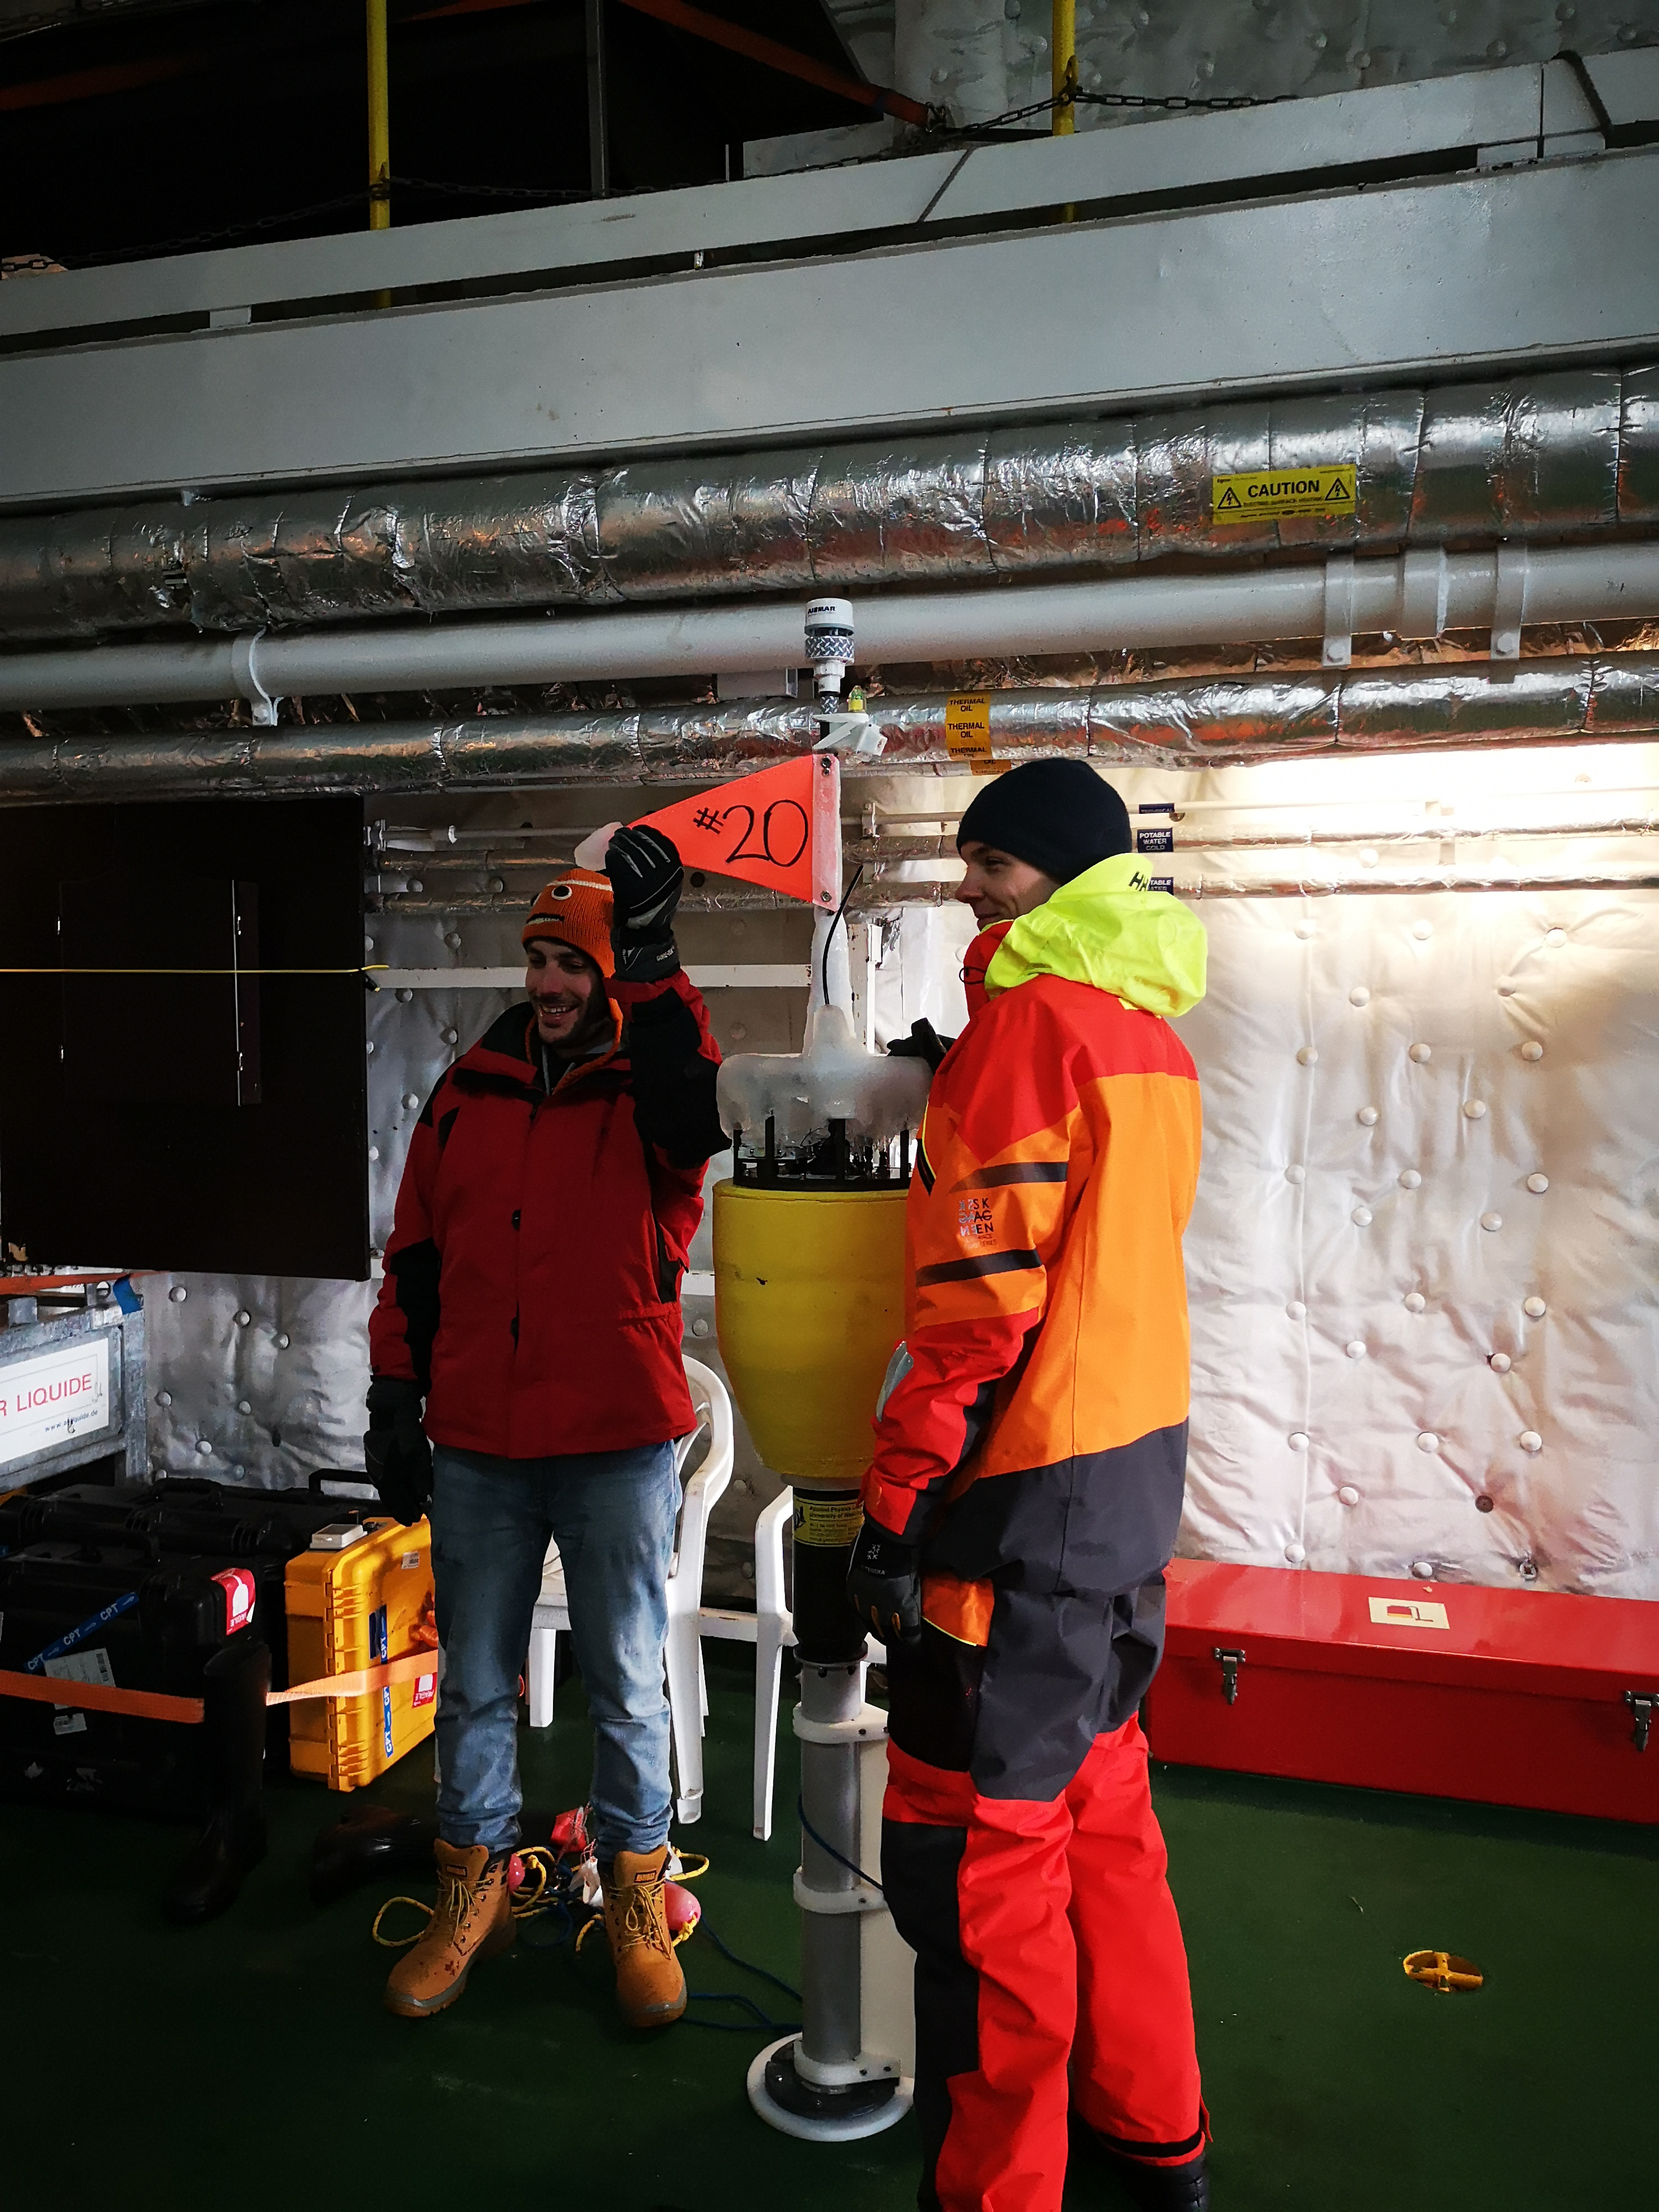
\includegraphics[width = 7cm]{swift_fail.jpg}
	\caption{During the 2019 SCALE winter expedition, a SWIFT device was retrieved early due to lost communication with the host. This failure was attributed to a build up of ice along the the rim from ocean spray. Photo taken by author.}
	\label{fig:swift_fail}
\end{figure}

Finally, \textcite{vichi2019effects} discuss the findings surrounding the failure of the first WIIOS system. \textcite{vichi2019effects} observed a major cyclonic event. The cyclone formed on  2 July 2017 and achieved lysis on 5 July 2017 which coincided with the buoy deployment. Following the event, four more cyclonic events were recorded with three explosive cyclones \cite{vichi2019effects} characterising a change of pressure over 24 hours. During this time, \textcite{vichi2019effects} observed winds speeds of up to $33$ $m \text{ }s^{-1}$ while noting that the air temperatures had increased to values "close to melting" \cite{vichi2019effects}. Additional observations found an increase in significant wave height in the activity. These conditions indicate deformation \cite{vichi2019effects} which may have subjected the buoys to forces experienced by \cite{doble2017robust} during their Arctic deployment which were verified against the temperature and pressure readings of the second WIIOS during the cyclonic event. The buoys were deployed close to the ice edge exposed to greater open ocean processes and cyclonic activities than other semi-consolidated and consolidated regions \cite{vichi2019effects}. As a result, air advection, storms and large wave movement delay the consolidation of sea ice considerably \cite{vichi2019effects}. Hence, the ice floes were more likely to experience rafting, ridging \cite{icedefinition1992}, extended flooding, and freezing over which may have caused the failures of the WIIOS buoys.

\subsection{Overall cost}
\label{subsec:sec2_overallcost}
Finally a key factor of buoy development is the cost and weight of the overall device. Additionally, devices are still deployed manually by manned teams. Such techniques involve deployments from on-ship cranes \cite{alberello2019drift,kohout2015device}, or by setting foot on the deployment site \cite{planck2019evolution,rabault2019open}. Additionally, \textcite{doble2017robust} deployed buoys by transporting them on a twin otter aircraft and installing them on arrival. This shows that the weight and form factor of the device can impact the ease of deployment as well as where the device can be deployed. The table below provides insight into the quoted price and development cost of each device in order to understand how expensive the current state of the art is.
\begin{table}[H]
	\centering
	\caption{Comparison of price and wieght of each device according to the published literature or commercial listing. Weight provides an indicator of the ease of handling whereas price provides an indicator of affordability. Prices have been converted to South African Rand (R)  online \cite{usdcoversion}where applicable while weight has been converted to Kg. "Not Reported"  or "N/R" is given where a value could not be obtained.}
	\label{tab:device_price}
	\small
	\begin{tabular}{|l|l|l|}
		\hline
		\textbf{Device Name:} & \textbf{Weight (Kg):} & \textbf{Price} \\
		\hline
		WIIB & 4.5 & R30,200.00\\
		\hline
		WIIOS & N/R & N/R \\
		\hline
		NDWB & 150 & N/R \\
		\hline
		SKIB  & N/R &  R39,784.40\\
		\hline
		SWIFT & 30 & N/R \\
		\hline
		SIMB & 34 & R58,909.30 \\
		\hline
		Polar ISVP & 11.34 & R52,119.00 \\
		\hline
		UptempO & 105 & R863,686.00 \\
		\hline
		Trident & 0.42 & R30,524.70 \\
		\hline
	\end{tabular}
\end{table}

Table \ref{tab:device_price} shows the current cost of in situ sensing devices. The cheapest wave sensing device is the WIIB at R30,200.00 thereby showing that \textcite{rabault2019open} succeeded in developing a feature-rich device for a cost relatively lower than the current state. Also included in the price comparison is a version of the Polar ISVP for deployment on ice floes called the UpTempo. This device is the lowest cost efficient device at R863,686.00 with only a GPS, pressure sensor and temperature sensor. This shows that in order to provide a cost effective solution, a new device will have to cost less than R30,200.00 however, this can be possible through the use of open-source and off-the-shelf solutions \cite{bonvoisin2017source}.\par
\newpage
\section{Subsystem Overview}

This section focuses on the subsystem analysis and component selection for each system. As stated previously, each buoy was created with a unique objective shown in table \ref{tab:device_deployment}. These objectives have influenced the sensor selection, topology and layout of the overall subsystems. In addition, the device designs choices have been influenced objectives for developing new in situ technologies by \textcite{kennicutt2016delivering} as the device developers have factored in power consumption \cite{kohout2015device}, ease of use and deployment \cite{rabault2019open}, long-term operation \cite{doble2017robust},cost \cite{planck2019evolution,rabault2019open} and availability of infrastructure \cite{doble2017robust} over and above functionality. For example WIIB was developed using open-source hardware \cite{rabault2019open} in order to increase access to readily available technology while WIIOS was developed using off-the-shelf components \cite{kohout2015device} to create a cost effective device. From table \ref{tab:device_deployment} we saw that the principle measurements of each device share the following measurement objectives:

\begin{enumerate}
	\item Ice drift
	\item Wave data/Wave in Ice data
	\item Ambient temperature
	\item Atmospheric pressure 
\end{enumerate}

The following sections discuss how these objectives have influenced sensor selection for each of these measurements as well as the hardware, and software strategies implemented to achieve these objectives.

\subsection{Processing capabilities}

The processing capabilities of each device facilitate the functionality of each buoy. A strong processor allows for the implementation of in-situ data processing and wave analysis algorithms \cite{kohout2015device,rabault2019open}. Additionally, due to the bandwidth constraints mentioned in section \ref{ch2:sec_remote}, some devices require data compression algorithms to allow the data to fit in the transmission buffers. The functionality of these devices has been made possible through the use of microprocessors.

\begin{figure}[H]
	\centering
	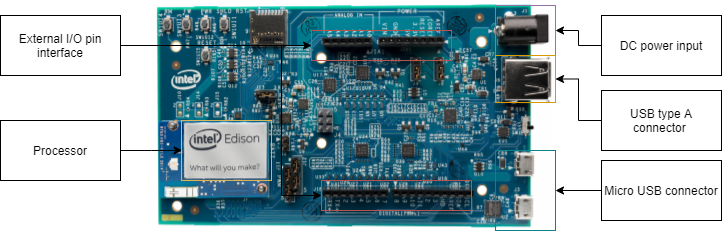
\includegraphics[width = 0.9\textwidth]{edison.png}
	\caption{Diagram of a typical microprocessor (yellow) on a development board. This device is an Intel Edison which was used as the main processor \textcite{kohout2015device} for the WIIOS. The development board allow for fast prototyping and integration into projects. The processor interface with external peripherals through physical input/output pins (Red) and contains standard serial communication ports such as USB (orange), micro USB (teal) and a connector for external voltage (purple). Image source: \cite{edison} }
\end{figure}

These are programmable integrated circuits that contain processing elements \cite{subham2018micro} and form the basis of microcontrollers and microcomputers \cite{crisp2003introduction}. These components are small and are increasingly becoming integrated into affordable, widely available components such as Raspbery Pis and Arduinos \cite{rabault2019open}. The table below shows a comparison of processors and topological implemented in each design

\begin{table}[H]
	\centering
	\caption{Comparison of the processing strategy implemented by each device. Multiple processors have been used in a selection of devices hence included in the comparison is the number of processors used and the type of processor used as well as the function of each processor }
	\label{tab:device_process}
	\setlength{\extrarowheight}{5pt}
	\resizebox{\textwidth}{!}{%
		
		\begin{tabular}{|l|>{\centering\arraybackslash}m{3cm}|>{\raggedright\arraybackslash}m{5cm}|l|}
			\hline
			\textbf{Device name} & \textbf{Number of processors} & \textbf{Processor name} & \textbf{Function} \\
			\hline
			\multirow{3}{*}{WIIB}& \multirow{3}{*}{3} & ATMega 328P & Low power unit \\ \cline{3-4} & & Arduino Mega 2560 & Data Logger \\ \cline{3-4} && Raspberry Pi Zero & Wave processing \\
			\hline
			\multirow{2}{*}{WIIOS} & \multirow{2}{*}{2} & Intel Edison dual core & Wave processing \\ \cline{3-4}&& ATMega 328P & Low power unit \\
			\hline
			NDWB & 1 & ACME Systems Fox G20 & Power control \\
			\hline
			\multirow{2}{*}{SKIB} & \multirow{2}{*}{2} & EFM32-M3 & Wave spectral processing \\ \cline{3-4} && Unspecified processor & Power control \\
			\hline
			SWIFT & 1 & Sutron Xpert & Data processing \\
			\hline
			SIMB & 1 & ATSAMD21G18 & Data processing control \\
			\hline
			Polar ISVP & 1 & Global Platform Transceiver Controller (GPTII)\footnotemark[1] & Data processing and control \\
			\hline
			\multirow{2}{*}{Trident} & \multirow{2}{*}{2} & Unnamed microprocessor & Data processing \\ \cline{3-4} && Unnamed low power unit & power control \\
			\hline	
	\end{tabular}}
\end{table}

\footnotetext[1]{Developed by \textcite{uptempo}$^{\text{TM}}$}
From table \ref{tab:device_process}, we can see that each device has been developed either with a single, powerful processor or with multiple, low powered processors. NDWB for instance builds its system around the dominant sensor i.e. the AHRS IMU with a single processor controlling all the peripherals as well as allowing for data processing. Drift loggers such as Trident, and Polar ISVP feature sparser sets of electronics with smaller, lower-powered processors for power control and peripheral control, In contrast, WIIOS and WII Buoy compartmentalise subsystems with a cluster of processors handling different aspects from the buoy. This shows a focus on computation rather than sensing as multiple controllers are used to free the main processor for implementing advanced digital signal processing. SWIFT Buoy appears as the outlier as the system is built around a dedicated data logger i.e. The Sutron Xpert with an integrated processor and satellite communication link abstracting data processing strategies on the buoy side. The SIMB buoy has the most advanced and largest number of sensors of all the buoys. A commonality among the buoys is the use of off the shelf components and processors. Another predominant feature, the GPS is an Adafruit MTK339 as well as SAMD Chips, Raspberry Pis and Arduino boards whereas, for Trident and MetOcean, more expensive solutions are used. This shows that developers have opted for ready-made that components that are auxiliary to the main measurements. This should explain why some components on a system are more advanced than others.



\subsection{Measurement of wave data using inertial measurement systems}

Typical wave state estimation are derived from calculating wave parameters such as significant wave height and dominant wave frequency \cite{williams2013wave}. Additionally, Wave data can be analyzed in terms of its power spectral density. The two main methods for wave data analysis presented in this section are the Kuik Method and the Welch-Earle Method. Further explanations can be found in Appendix \ref{kuik}. Both approaches rely on a discrete time series of inertial data from a device with 3 axes of acceleration of 3 axes of rotation \cite{kuik1988method,earle1996nondirectional}.

\begin{figure}[H]
	\centering
	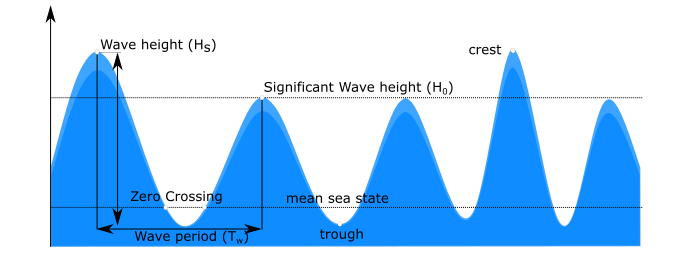
\includegraphics[width=\linewidth]{sea state diagram.png}
	\caption{Diagram showing the characterization of sea state through statistical methods described by \textcite{kuik1988method} and \textcite{earle1996nondirectional,welch1967use}. A wave consists of a maximum vertical point (crest) and a minimal vertical point (trough) with the distance between the two points referred to as the wave height ($H_0$). The period between consecutive crests of a similar frequency is referred to as the wave length and the point where a wave crosses the mean sea state level is the zero crossing. From a statistical analysis, the significant wave height is four times the average wave height measured from the spectral density over a period of time \cite{kuik1988method}. Diagram is based off the figure by \cite{seastatediag}.}
	\label{fig:seastatediag}
\end{figure}

Devices that measure wave parameters such as significant wave height, wave spectra or ocean states, incorporate a sensor that measures the vertical acceleration and roll, pitch, and yaw in discretised space \cite{earle1996nondirectional}. These parameters can be measured using an accelerometer for axial acceleration and a gyroscope for rotational velocity \cite{fong2008methods}. These devices are typically integrated circuits manufactured using micro electro-mechanical systems (MEMS) and are often combined to form an inertial measurement unit (IMU) allowing for 6 axes of measurement from a single device \cite{fong2008methods}. IMUs can also be expanded to include a magnetometer which measures magnetic bearing in 3 axis\cite{ahmad2013reviews}.IMU selection is dependent on the following factors\footcite{ahmad2013reviews}:
\begin{enumerate}
	\item Package size
	\item Accuracy
	\item Response rate
	\item Degrees of freedom
\end{enumerate}

\begin{figure}[H]
	\centering
	\begin{subfigure}[t]{.3\textwidth}
		\begin{tikzpicture}
			\node[anchor=south west,inner sep=0] (image) at (0,0) { 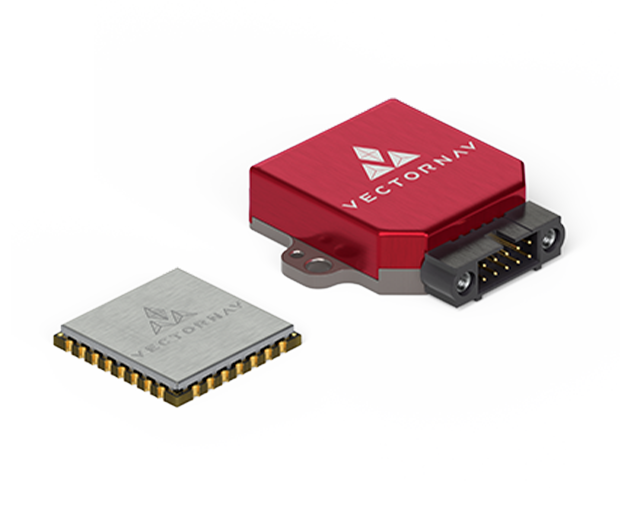
\includegraphics[width = 4cm, height = 6cm]{vn-100-smd-rugged_new.png}};
			\begin{scope}[x={(image.south east)},y={(image.north west)}]
				\draw[color=black, ultra thin,fill=white] (0.0,0.0) rectangle (0.21,0.16) node[pos=.5] {A};
			\end{scope}
		\end{tikzpicture}
	\end{subfigure}
	\hfill
	\begin{subfigure}[t]{.3\textwidth}
		\begin{tikzpicture}
			\node[anchor=south west,inner sep=0] (image) at (0,0) { 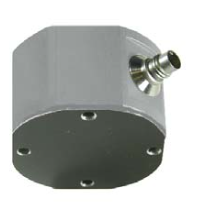
\includegraphics[width = 4cm, height = 6cm]{servokbeam.PNG}};
			\begin{scope}[x={(image.south east)},y={(image.north west)}]
				\draw[color=black, ultra thin,fill=white] (0.0,0.0) rectangle (0.21,0.16) node[pos=.5] {B};
			\end{scope}
		\end{tikzpicture}
	\end{subfigure}
	\hfill
	\begin{subfigure}[t]{.3\textwidth}
		\begin{tikzpicture}
			\node[anchor=south west,inner sep=0] (image) at (0,0) { 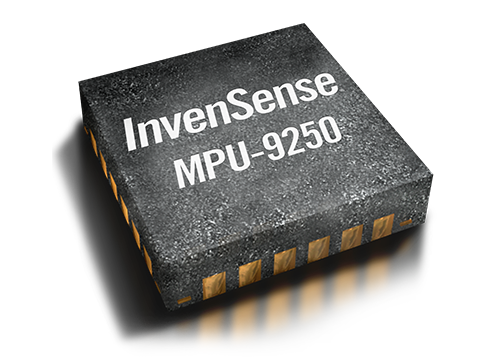
\includegraphics[width = 4cm, height = 6cm]{rp-mpu-9250.png}};
			\begin{scope}[x={(image.south east)},y={(image.north west)}]
				\draw[color=black, ultra thin,fill=white] (0.0,0.0) rectangle (0.21,0.16) node[pos=.5] {C};
			\end{scope}
		\end{tikzpicture}
	\end{subfigure}
	\hfill
	\label{fig:imus}
	\caption{Diagram showing examples of the different types of inertial measurement systems (IMUs) available for commercial use such as (A) an Attitude Heading Reference System (AHRS) VN100 \cite{vn-100} used by \cite{rabault2019open}, (B) an analog capacitive accelerometer 8330B3 Servo-KBeam accelerometer used by \cite{kohout2015device} \cite{kistlerIMU} and (C) a 9 degree of freedom MPU9520 \cite{mpu9520} used by \cite{kohout2015device}. }
\end{figure}

\textcite{ahmad2013reviews} show that package size can limit the applications of the IMU. Additionally, IMUs require careful calibration and filtering in order to reduce the effects of bias offsets as well as low and high frequency drift \cite{fong2008methods}. More advanced filtering methods have been developed to improve the accuracy of IMUs such as Kalman filters \cite{simon2001kalman}  for positional estimates or Real-Time Kinetic Fusion (RTK) for velocity \textcite{meng2014optimal}. While important to the integrity of IMU data, these methods are usually implemented in software which is discussed in the upcoming sections. Finally, the degrees of freedom (DoF) influences the application of the IMU. The magnetometer is used to improve the accuracy of the gyroscope measurement and account for low frequency noise (drift) \cite{ahmad2013reviews}. However, removing the magnetometer is sensitive to magnetic distortion which can affect the measurements. \textcite{kohout2015device} encountered magnetic distortion during the SIPEX II deployments in September 2012 which rendered the magnetometer readings useless. In this section, the IMU is integral to deriving a time-series representation of inertia to calculate wave data as described above however, another application relevant to the literature is using IMUs to improve navigation \cite{ahmad2013reviews}. An IMU can be coupled with a Global Positioning System (GPS) device to determine position in areas with poor signal which can assist greatly with determine ice drift (discussed in section \ref{sec:ch2_drift}). Based on these considerations, table \ref{tab:imu_component} shows the IMU component selection for each device.
 
%TODO add table

\begin{table}[H]
	\centering
	\setlength{\extrarowheight}{5pt};
	\caption{Comparison of the inertial measurement systems selected for each device showing the sensors included as well as the degrees of freedom.}
	\label{tab:imu_component}
	\resizebox{\textwidth}{!}{%
		\begin{tabular}{|l|l|l|c|l}
			\cline{1-4}
			\textbf{Device name} & \textbf{Inertial Measurment Unit} & \textbf{Sensors} & \textbf{Degrees of freedom} &  \\ \cline{1-4}
			\multirow{3}{*}{WIIB} & \multirow{3}{*}{VN-100} & Accelerometer & \multirow{3}{*}{9} &  \\ \cline{3-3}
			&  & Gyroscope &  &  \\ \cline{3-3}
			&  & Magnetometer &  &  \\ \cline{1-4}
			\multirow{4}{*}{WIIOS} & 8330B3 Servo-KBeam & Vertical Acceleration & 1 &  \\ \cline{2-4}
			& \multirow{3}{*}{MPU9250} & Accelerometer & \multirow{3}{*}{9} &  \\ \cline{3-3}
			&  & Gyroscope &  &  \\ \cline{3-3}
			&  & Magnetometer &  &  \\ \cline{1-4}
			\multirow{3}{*}{NDWB} & \multirow{3}{*}{IG-500N} & Accelerometer & \multirow{3}{*}{9} &  \\ \cline{3-3}
			&  & Gyroscope &  &  \\ \cline{3-3}
			&  & Magnetometer &  &  \\ \cline{1-4}
			SKIB & LIS3DH & Accelerometer & 3 &  \\ \cline{1-4}
			\multirow{3}{*}{SIMB} & \multirow{3}{*}{BNO055} & Accelerometer & \multirow{3}{*}{9} &  \\ \cline{3-3}
			&  & Gyroscop &  &  \\ \cline{3-3}
			&  & Magnetomer &  &  \\ \cline{1-4}
			Polar ISVP & None & - & - &  \\ \cline{1-4}
			Trident & None & - & - &  \\ \cline{1-4}
		\end{tabular}
		}
\end{table}

As mentioned previously, systems such as WIIOS and WIIB have built their purpose around wave measurements and therefore have specified high powered, high accuracy IMUs for wave measurements. However, WIIOS buoy separates itself from WIIB by having a cheaper complimentary 9 dof IMU to complement the measurements \cite{kohout2015device}. SWIFT Buoy and the NDWB buoy use an integrated system known as an Inertial Navigation System (INS) with the former containing an SBG Elipse AHRS \cite{thomson2012wave} and the latter containing a IG-500-A1G2 \cite{doble2017robust}. This device contains a GPS and an Onboard processor for RTK fusion and Kalman filtering whereas other devices use an external processor for filtering. The SIMB Buoy is the only buoy on the list that has an IMU for non-wave related measurements. It uses a cheaper Bosch BNO055 which is used solely for measuring the orientation of the device.

\subsubsection{Software processing}

An IMU is a power device however extensive software proccessing is required to extract key parameters \cite{ahmad2013reviews}. Examples of software processing algorithms are shown in \textcite{kuik1988method} and \textcite{earle1996nondirectional}\footnote{See Appendix \ref{welchearl}.} for wave processing algorithms. Additionally, as mentioned previously, advanced filtering techniques are required to reduce the effects of low and high frequency noise. In this subsection the software processing strategy for each device given for extracting the desired parameters shown in table \ref{tab:device_deployment}.

\begin{table}[H]
	\centering

	\caption{Comparison of sampling strategies implemented in each device. This includes the desired measurands, sample rate and sample period of each IMU session}
	\label{tab:device_imumeasure}
	\setlength{\extrarowheight}{5pt}
	\resizebox{\textwidth}{!}{%

		\begin{tabular}{|l|l|l|l|}
			\hline
			\textbf{Device name} & \textbf{Degree of Freedom used} & \textbf{Sample rate} & \textbf{Sample Period} \\ \hline
				\multirow{3}{*}{WIIB} & Vertical Acceleration & \multirow{3}{*}{10 Hz} & \multirow{3}{*}{25 minutes} \\ \cline{2-2}
				& Pitch &  &  \\ \cline{2-2}
				& Roll &  &  \\ \hline
				\multirow{4}{*}{WIIOS} & 3-axis acceleration & \multirow{4}{*}{2 Hz} & \multirow{4}{*}{11 minutes} \\ \cline{2-2}
				& 3-axis gyroscope &  &  \\ \cline{2-2}
				& 3-axis magnetometer &  &  \\ \cline{2-2}
				& Vertical  analog acceleration &  &  \\ \hline
				\multirow{5}{*}{NDWB} & 3-axis acceleration & \multirow{5}{*}{1 Hz} & \multirow{5}{*}{Continuous} \\ \cline{2-2}
				& 3-magnetometer &  &  \\ \cline{2-2}
				& heave &  &  \\ \cline{2-2}
				& roll &  &  \\ \cline{2-2}
				& pitch &  &  \\ \hline
				SKIB & 3-axis acceleration & 25 & 10 minutes \\ \hline
				\multirow{3}{*}{SWIFT} & 3-axis acceleration & \multirow{3}{*}{5} & \multirow{3}{*}{9 minutes} \\ \cline{2-2}
				& Tilt &  &  \\ \cline{2-2}
				& Horizontal Rotation &  &  \\ \hline
				\multirow{2}{*}{SIMB} & Tilt & \multirow{2}{*}{-} & \multirow{2}{*}{-} \\ \cline{2-2}
				& Orientation &  &  \\ \hline
			\end{tabular}
			}
		\end{table}

\textcite{rabault2019open} extract wave parameters by passing the raw time series data through an Extended Kalman Filter running at 800 Hz then through a low pass filter. Wave spectral data is calculated using the method by \textcite{earle1996nondirectional} where Co-spectra was calculated using the method by \textcite{kuik1988method}. Significant wave height wass calculated through double integration using a Fast Fourier Transform. sampling is performed at 10 Hz to satisfy the nyquist sampling criteria for open ocean waves as described in \cite{rabault2019open,earle1996nondirectional}.

\textcite{kohout2015device} however, opted for a reduced sampling rate of 2 Hz over a shorter sample time. This was achieved by oversampling IMU data at 640 Hz then down-sampling the data through a multistage decimator \cite{kohout2015device}. Before each decimation, data was filtered using a Butterworth filter at 8 Hz with a cut-off frequency of 2 Hz, then once again at 40 Hz. Significant wave height is calculated by double integration using the Welch-Earl method \cite{earle1996nondirectional,welch1967use} multiplying the transformed data set by a response weighted function to remove low frequency drift. Finally, the Longuet-Higgens parameters are calculated thereby characterizing wave in ice activity.

\textcite{doble2017robust} did not apply any data processing algorithm to the raw time series as it is transmitted directly over iridium. However, the raw time series is filtered using an Extended Kalman Filter running at 10 Hz.

The SKIB collects data from a sample window which is processed using a classical RC filter to attenuate frequencies below 0.04 Hz.Thereafter, \textcite{earle1996nondirectional} spectra and Co-spectra calculation are then applied.

The SWIFT buoy is the only device that used multiple sensor types for sea state calculation. Additionally, data was collected more frequently in short intervals (9 minute sample periods every 12 minutes) which include Doppler profiles, camera images and IMU data. The inertial navigation system (INS) outputted a real-time kinematic (RTK) fusion data set where IMU data was passed through a Coning \& Sculling Extended Kalman Filter running at 1 KHz \cite{thomson2012wave} while the doppler profiler was sampled at 8 Hz. Turbulence profile was calculated through time-averaging and data fitting of the Doppler profile. Then, the ocean current state was calculated using the Stokes drift equation over a time-averaged velocity series. Finally, wave data was calculated  through image processing from a still of the sea state taken from an onboard camera.

\par{SIMB}

The SIMB uses the IMU in a non-critical manner. The device transmits tilt and orientation metadata \cite{planck2019evolution} describing the current status of the SIMB. While no method has been described by \textcite{planck2019evolution} to calculate tilt, it can be achieved by measuring the orthogonal acceleration values over an angle of ration and taking the inverse tangent of the resulting value for each axis \cite{tuck2007tilt}.


Therefore IMUs are integral for performing sea state calculations and measuring wave spectra, a sufficient processor is required to filter and process the data therefore, significant consideration should be given to coupling a powerful processor with a sufficiently powerful inertial measurement unit.

\subsection{Measurement of Ice drift using GPS}
\label{sec:ch2_drift}

This sections discusses the technology and techniques used for determining ice drift. The predominant approach towards understanding modeling ice drift is by using the techniques presented by \textcite{hibler1979dynamic}\footnote{See Numerical Modeling in Appendix \ref{app:modelling}} where kinematic data is used to study ice drift dynamics and calibrate the ice drift model. Additionally, \textcite{lepparanta2001sea} present two methods for collecting ice drift data. The first method utilises measurement beacons are attached to the ice floes and used to track trajectories. The second method uses imaging devices such as radar, and satellites to determine ice displacement \cite{lepparanta2001sea}.\par

\begin{figure}[H]
	\centering
	\begin{subfigure}[t]{.3\textwidth}
		\begin{tikzpicture}
			\node[anchor=south west,inner sep=0] (image) at (0,0) { 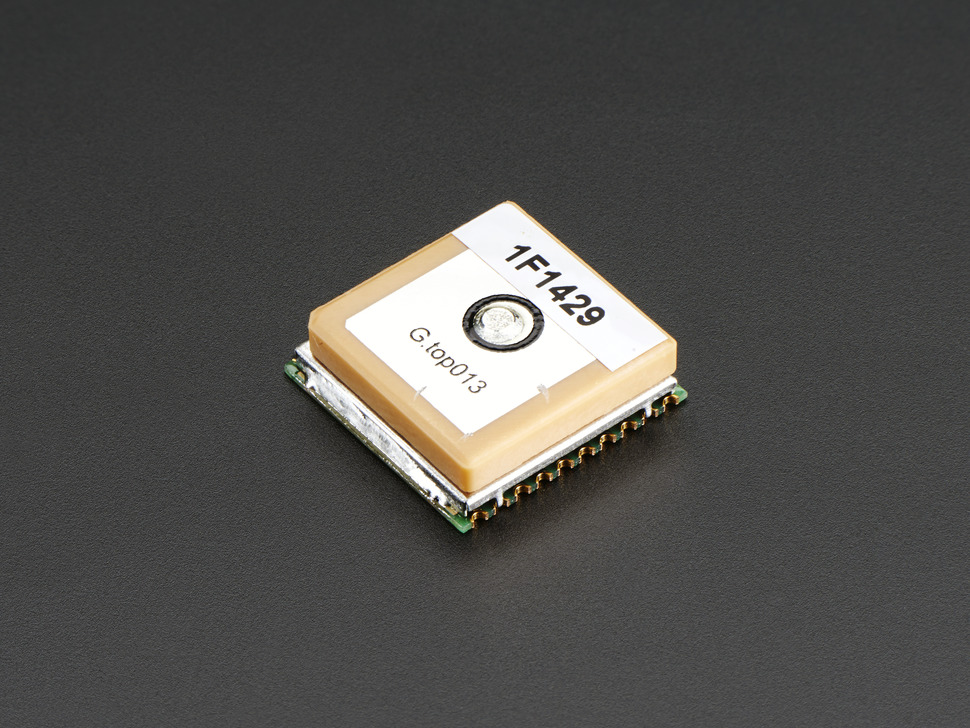
\includegraphics[width = 4cm, height = 6cm]{mtk3339.jpg}};
			\begin{scope}[x={(image.south east)},y={(image.north west)}]
				\draw[color=black, ultra thin,fill=white] (0.0,0.0) rectangle (0.21,0.16) node[pos=.5] {A};
			\end{scope}
		\end{tikzpicture}
	\end{subfigure}
	\hfill
	\begin{subfigure}[t]{.3\textwidth}
		\begin{tikzpicture}
			\node[anchor=south west,inner sep=0] (image) at (0,0) { 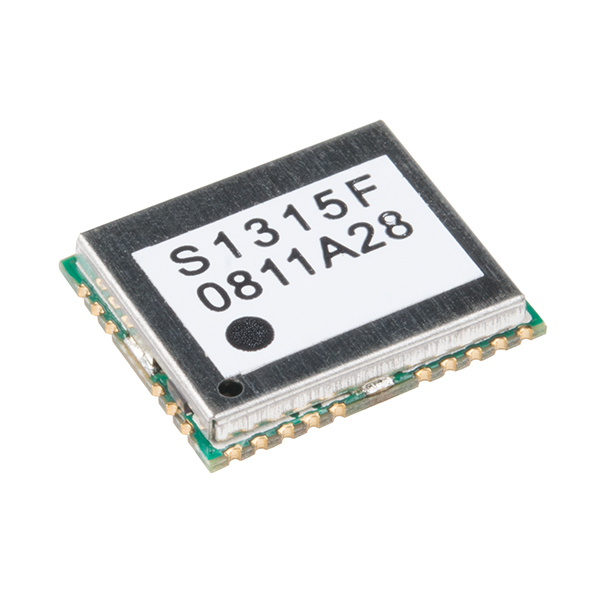
\includegraphics[width = 4cm, height = 6cm]{skytraq.PNG}};
			\begin{scope}[x={(image.south east)},y={(image.north west)}]
				\draw[color=black, ultra thin,fill=white] (0.0,0.0) rectangle (0.21,0.16) node[pos=.5] {B};
			\end{scope}
		\end{tikzpicture}
	\end{subfigure}
	\hfill
	\begin{subfigure}[t]{.3\textwidth}
		\begin{tikzpicture}
			\node[anchor=south west,inner sep=0] (image) at (0,0) { 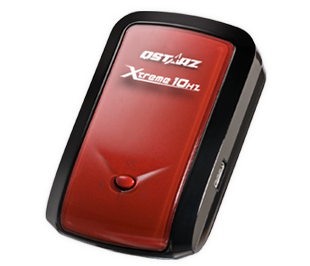
\includegraphics[width = 4cm, height = 6cm]{BT-1000ex-310-1.png}};
			\begin{scope}[x={(image.south east)},y={(image.north west)}]
				\draw[color=black, ultra thin,fill=white] (0.0,0.0) rectangle (0.21,0.16) node[pos=.5] {C};
			\end{scope}
		\end{tikzpicture}
	\end{subfigure}
	\hfill
	\label{fig:device_gps}
	\caption{Diagram showing examples of the different types of global positioning devices available for commercial use such as (A) MTK3339 (image source: \cite{mtk3339}) , (B) SkyTraq S1351R (image source: \cite{s1315F}) (C) Qstarz BT-Q1000eX (image source: \cite{BTQ1000EX})  }
\end{figure}
The discussion of modern technology for ice observations from chapter \ref{sec:ch1.section1} showed that observations from satellites such as OSI-SAF and METSAT are unsuitable for measurements \cite{lepparanta2001sea,galin2011validation} due to their low spatial resolutions. Hence, a need arises for in situ drift measurement devices. Global positioning systems (GPS) have been the standard for ice drift measurements \cite{lepparanta2001sea} as they are capable of measuring data at relatively high temporal resolutions ranging from 15 minutes \cite{alberello2019drift} to 25 minutes \cite{rabault2019open} as opposed to the limit of 3 hours \cite{alberello2019drift}. This section provides an overview of GPS technology and how the devices have implemented it for measuring positional or drift data.

\subsubsection{Overview of GPS}

The principles that govern GPS have remained unchanged since its inception in 1973 \cite{spilker1996global}. The system consists of a satellite constellation that constantly broadcast their estimated position. A GPS device determines its position by matching a user-generated signal to that of four received satellites and comparing the phase difference to an on-board crystal oscillator \cite{spilker1996global}. This technique is called ranging and four satellites spread in a uniform geometry will allow for a device to calculate latitude, longitude, altitude and time to a relative degree of accuracy. The number of unknown signals correlates to the number of satellites required. Generally, a GPS device will have a lesser degree of accuracy than the satellites. Hence, an incoming signal can be used to correct the device's clock \footnote{provided altitude or time are already known \cite{spilker1996global}}.To accurately predict the satellite's trajectory, satellite ranging is performed by a network of global monitoring which calculate the future position and send it back to the satellite. GPS signals are transmitted on two frequencies: 1575.42 MHz and 1227.46 MHz\cite{spilker1996global}. These are synchronously generated signals and allow a device to correct for ionospheric distortion. These bands carry modulated signals which are as follows: \cite{spilker1996global}


\begin{enumerate}
	\item Clear Acquisition Code:  This is a short code transmitted at 1.023 MHz and is used to request the Standard Positioning Service or SPS.
	\item Precise (P) Code: this is a much longer acquisition code. This signal is transmitted at 10.23MHz which is 10 x the rate of a CA code. This results in a much more accurate signal with less noise. This signal allows for the acquisition of Precise Positioning Service. However, this service is not available to unauthorized users and cannot be spoofed. As a result, this signal requires additional decryption.    
\end{enumerate}

\textcite{spilker1996global} also mention that military operators can degrade GPS signals which result in decreased accuracy from 20 m up to 100 m. The reduction of these accuracies requires differential GPS techniques, however, due to the scope of this projects, this section will not be explored any further.Finally, once the acquisition signal is transmitted, the GPS device begins modulating at 50 bit/s. This allows the satellite to transmit its position as well as clock correction information to the device.\par

The GPS satellite constellation consists of 24 GPS satellites. These are configured into three rings of eight satellites orbiting at different latitudes. These orbital altitudes were selected as 10.98 Nautical Miles \cite{spilker1996global}. This altitude was chosen to optimise user visibility with the number of crossings over United Sates ground stations, and cost of launching the satellites \cite{spilker1996global}. These satellites carry onboard atomic clocks for stability at $1\times10^{13}$ resolution. This allows for extremely accurate signaling as well as allowing for much more predictable time and position signals \cite{spilker1996global}. To achieve this, these atomic clocks are made out of either Cesium or Rubidium. Also, a frequency correction at $4.5\times10^{10} \text{ } Hz$ is provided to correct for relative shifts. \par

\subsubsection{GPS Error Modeling}

As mentioned in the previous section,GPS signal accuracy is greatly affected by earth effects and satellite distribution. The main source of distortion is attributed to the earth's ionosphere \cite{spilker1996global}. The ionospheric free electronics cause a delay in the modulated signal which is proportional to the sum of electrons along the signal's trajectory and inversely proportional to the signal's frequency squared. This delay is modeled as the product of a theoretical $90^\circ$ delay (Zenith delay) and a function of the elevation angle (obliquity factor). This results in a ratio of between 1.0 to 3.0 at small elevation angles \cite{spilker1996global}. This results in delays of 3 m (often at night) to 20 m (after midday).These delays result in errors in positional accuracy as shown in figure \ref{fig:DOP_effects} which can increase the measurement confidence interval resulting in an unreliable positional reading \cite{spilker1996global}. Fortunately,These delays are usually resolved by satellite correlated positions.

\begin{figure}[H]
	\centering
	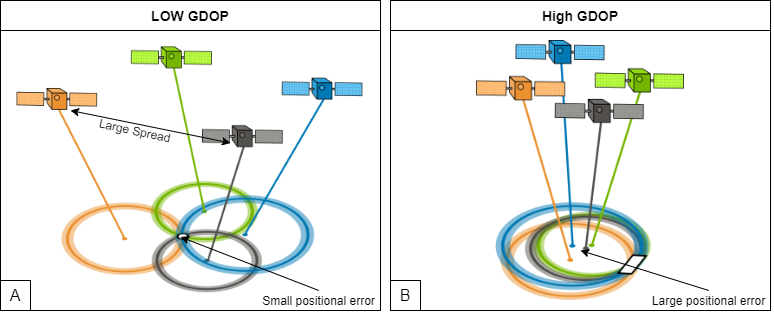
\includegraphics[width =\linewidth]{DOPeffect.png}
	\caption{Diagram showing how satellite distribution affects the positional estimation. GNSS Satellites have an associated inaccuracy which is represented by the circles. Locking on to more than one satellite reduces these inaccuracies by interpolating the position from the phase differences between satellites. This value is greatly affected by the spread of satellites as a larger spread results in a more accurate positional estimate (A) while a shorter satellite spread results in a less accurate positional estimate. A measure of this inaccuracy is called the dilation of procession (DOP). Figure was adapted from images by \cite{GISGeo2020DOP} for A and B.}
	\label{fig:DOP_effects}
\end{figure}

 Correction can be performed in one of two ways:
\begin{enumerate}
	\item Transmission of Ionospheric model parameters as part of the message to the device and calculating the offset using that
	\item Using the two previously mentioned transmission frequencies directly measuring the delays in each broadcast frequency and estimating the position using the equation:\cite{spilker1996global}
	\begin{equation}
		1.546(delay_{L1} - delay_{L2})
	\end{equation}
\end{enumerate}

Navigation errors are characteristic of GPS performances. These errors are affected significantly by satellite spread and ranging errors. Assuming the incoming signal is uncorrelated with a mean of zero, the RMS positional error is calculated as:
\begin{equation}
	RMS_{error} = (\text{Geometric Dilution})(\text{RMS Ranging errors})
\end{equation}

The geometric dilution is modeled by estimating the processional dilution of the spatial and temporal dimension measurements. This value estimates the quality of the GPS signal and is inversely proportional to the volume of the shape formed by 4 satellite \cite{jwo2001efficient}. \textcite{jwo2001efficient} outlines the procedure for the calculation of this value. Given a user's position on the earth, the distance from the user to the satellite is characterised by the equation:
\begin{equation}
	r =  s - u
\end{equation}
where $r$ is the distance from the user to the satellite, $s$ is the distance from the earth's centre to the satellite and u is the distance from the earth to the user. By measuring the propagation time from the user to the satellite, The absolute distance $||r||$ can be calculated and hence, the pseudo-range can be calculated as
\begin{equation}
	\rho_i = ||s_i-u||+ct_b + v_{\rho_i}
\end{equation}
where $\rho_i$ is the pseudorange for satelite i, c is the speed of light, $t_b$ is  the clock offset and $v_{\rho_i}$ is the noise of the pseudorange measurement and:
\begin{equation}
	||s_i-u|| = \sqrt{(x_i - x_u)^2+(y_i-y_u)^2+(z_i-z_u)^2} \text{ for } i \in 1,2,3...N \label{los}
\end{equation}
where $N$ is the number of satellites and $(x_i,y_i,z_i)$ is the 3 dimensional position of satellite $i$. This represents a non-linear relationship for the line of sight of a satellite.  \textcite{jwo2001efficient} explains that by creating a Taylor series centered on a nominal user position $(\hat{x_n},\hat{y_n},\hat{z_n})$ and ignoring the higher terms \cite{jwo2001efficient}. It then follows that:
\begin{equation}
	\Delta\rho_i = \rho_i - \hat{\rho_i} = e_{i1}\Delta x_u + e_{i2}\Delta x_u +  e_{i3}\Delta z_u
\end{equation}

The terms $e_{ij}$ represent the line of sight vector $E_i$ whereas the term $\hat{\rho_i}$ is the pseudo-range at the nominal user's position. It follows that the vector $E_i$ can be calculated as follows \cite{jwo2001efficient}.
\begin{subequations}
	\begin{align}
		e_{i1} = \frac{\hat{x_n} - x_i}{\hat{r_i}}\\
		e_{i2} = \frac{\hat{y_n} - y_i}{\hat{r_i}}\\
		e_{i3} = \frac{\hat{z_n} - z_i}{\hat{r_i}}\\
		\hat{r_i} = \sqrt{(\hat{x_n} - x_i)^2+(\hat{y_n} -y_i)^2+(\hat{z_n} -z_i)^2}
	\end{align}
\end{subequations}

Given $n$ satellites, the equation \eqref{los} can be written as a matrix with the following form:
\begin{equation}
	\textbf{z} = \textbf{Hx}+ \textbf{v}
\end{equation}
\begin{equation}
	\Delta \rho _i = \begin{bmatrix}
		\Delta \rho_1 &  \Delta \rho_2 &  \Delta \rho_3 & ... & \Delta \rho_n
	\end{bmatrix} 
\end{equation}
where 
\begin{subequations}
	\begin{align}
		\textbf{H} = \begin{bmatrix}
			e_{11} & e_{12} & e_{13}& 1 \\
			e_{21} & e_{22} & e_{23}& 1 
			\\
			e_{31} & e_{32} & e_{33}& 1
			\\
			... & ... & ... &  1 
			\\
			e_{n1} & e_{n2} & e_{n3} & 1
		\end{bmatrix}\\
		\textbf{x} = \begin{bmatrix}
			\Delta x_u \\ \Delta y_u \\\Delta z_u \\ c\Delta t_b
		\end{bmatrix}\\
		\textbf{v} = \begin{bmatrix}
			v_{\rho_1}\\
			v_{\rho_2}\\
			v_{\rho_3}\\
			...\\
			v_{\rho_n}
		\end{bmatrix}
	\end{align}
\end{subequations}

The Matrix \textbf{H} is $n\times4$ where $n \geq 4$ to calculate all the parameters for GDOP \cite{jwo2001efficient}. We can then solve for the vector \textbf{x} by taking the psuedo inverse of H i.e $\hat{\textbf{x}} = (\textbf{H}^T\textbf{H})^{-1}\textbf{H}^t\textbf{z}$. Hence, given that the psuedo range is linearised, the quality of navigation is taken as the difference between the estimated position and the actual position \cite{jwo2001efficient}.
\begin{equation}
	\Tilde{\textbf{x}} = \hat{\textbf{x}} - x = (\textbf{H}^T\textbf{H})^{-1}\textbf{H}^Tv
\end{equation}
$E\{\Tilde{\textbf{x}}\Tilde{\textbf{x}}^T\}$ describes the covariance between the errors in the components of the estimated position \cite{jwo2001efficient} and is calculated as 
\begin{equation}
	E\{\Tilde{\textbf{x}}\Tilde{\textbf{x}}^T\} = (\textbf{H}^T\textbf{H})^{-1}\textbf{H}^TE\{\textbf{vv}^T\} (\textbf{H}^T\textbf{H})^{-1}\textbf{H}
\end{equation}
where $E\{\textbf{vv}^T\} = \sigma^2 I$. If all components of $\sigma$ are uncorrelated then the covariance becomes 
\begin{equation}
	E\{\Tilde{\textbf{x}}\Tilde{\textbf{x}}^T\} = \sigma^2(\textbf{H}^T\textbf{H})^{-1}
\end{equation}
and thus the GDOP factor can be calculated from the RMS values of $\sigma^2$ i.e.
\begin{equation}
	GDOP = \frac{\sqrt{\sigma_{xx}^2+\sigma_{yy}^2+ \sigma_{zz}^2+\sigma_{tt}^2}}{\sigma}
\end{equation} where $\sigma_{xx}^2$,$\sigma_{yy}^2$,$\sigma_{zz}^2$,$\sigma_{tt}^2$ are the RMS values of the x,y,z time components respectively. THe value GDOP can also be decomposed into the positional dilation of precision (PDOP), time dilation of precision (TDOP), horizontal dilation of precision HDOP, and vertical dilation of precision (VDOP) which characterise the effects satellite spread on the 3 dimensional position, time, horizontal position and altitude respectively.\par

Ranging errors are shown to come from 6 sources \cite{spilker1996global}:
\begin{enumerate}
	\item Satelite ephemeris
	\item Satelite clock
	\item Ionospheric group delay
	\item Trophospheric group delay
	\item Multipath scattering
	\item Hardware/software errors
\end{enumerate}

These errors need to be accounted for in order to produce an accurate, reliable position.

\subsubsection{GPS Component Selection}

The component selection for each device is shown in table \ref{tab:dev_gps} below.

\begin{table}[H]
	\centering
	\caption{Comparison between different GPS devices, sampled data and periods between samples implemented by each device.}
	\label{tab:dev_gps}
	\setlength{\extrarowheight}{5pt}
	\resizebox{\textwidth}{!}{% 
	\begin{tabular}{|l|l|l|l|}
		\hline
		\textbf{Device Name} & \textbf{GNSS Device} & \textbf{Data Sampled} & \textbf{Period between Samples} \\ \hline
		WIIB & MTK3339 & Geographical position & 25 minutes \\ \hline
		\multirow{2}{*}{WIIOS} & \multirow{2}{*}{MTK3339} & Latitude (decimal degrees) & \multirow{2}{*}{3 hours} \\ \cline{3-3}
		&  & Longitude (decimal degrees) &  \\ \hline
		NDWB & SkyTraq S1351R & Geographical position & 1 hour \\ \hline
		SKIB & MTK3339 & Geographical postion & 10 minutes \\ \hline
		\multirow{2}{*}{SWIFT} & \multirow{2}{*}{Qstarz BT-Q1000eX} & Geographical position & \multirow{2}{*}{200 ms} \\ \cline{3-3}
		&  & Horizontal velocity &  \\ \hline
		SIMB & MTK3339 & Geographical position & 1 hour \\ \hline
		Polar ISVP & Jupiter F2 Module & Geographical position & 3 hours \\ \hline
		\multirow{3}{*}{Trident} & \multirow{3}{*}{Unspecified GPS} & \multirow{3}{*}{Geographical position} & 0 - 5 minutes \\ \cline{4-4} 
		&  &  & 5 - 60 minutes \\ \cline{4-4} 
		&  &  & 1 - 24 hours \\ \hline
	\end{tabular}	
	}
	
\end{table}
Table \ref{tab:dev_gps} above shows the GPS receivers implemented in each system as well as measurements of interest. The most common gps is the MTK3339, a gps module developed by adafruit (cite). Additionally, all devices have fixed transmission periods between samples except the Trident buoy which has user configurable periods that can be set from a couple of minutes to full hours. Most devices use the GPS for positional location however, SWIFT buoy measures horizontal velocity in addition to vertical position\cite{thomson2012wave}. \textcite{thomson2012wave} justify this by stating that the accuracy of horizontal velocity measured by a gps is accurate enough ($\pm 0.5 \text{ }m\cdot s^{-1}$)to be used for determining the orbital motions of waves. \textcite{kohout2015device} and \textcite{rabault2019open} provide the measurements recorded by the GPS however, very little discussion is given regarding the performance of the device. \textcite{doble2017robust} showed that during their year long deployment, 14 buoys maintained a near perfect satellite signal acquisition however, software issues with the GNSS reciever resulted in a failure to obtain measurements in 5 systems. However, \textcite{doble2017robust} had implemented two-way iridium communication and were able to partially overcome this set back by transmitting commands that performed a software reset on the GPS receiver. Additionally, two devices lost signal for 6 days while another two devices lost signal for 62 days and 41 days respectively \cite{doble2013wave}. This shows that acquisition failures can cause temporal gaps in data and therefore, need to be reduced in order to provide robust data sets.

Each ice floe follows a unique trajectory \cite{lepparanta2001sea}  and individual trajectories combine to form a continuum. It has previously been believed that sea ice drift has been linked strongly to significant wave events \cite{alberello2019drift}. An experiment was conducted by \textcite{alberello2019drift} to measure the drift of sea ice during a cyclone event. Here it was found that wind velocity is the dominant driver of sea ice drift \cite{alberello2019drift} causing ice drifts of up to $0.75\text{ } m\cdot s^{-1}$ \cite{alberello2019drift}. Sea ice drift speed is extremely sensitive to sampling rates. \cite{alberello2019drift} where sampling rates of 6 hours can underestimate the ice velocity by 5\% \cite{alberello2019drift} and up to 20\% for 12-hour sample rates. The consequence is reduced, near unusable, estimates of sea ice velocity components as well as drag coefficient and wind factor estimates. High temporal resolutions are capable of capturing important, inter-daily activities such as ice oscillations. \textcite{alberello2019drift} state that to accurately capture Sea ice dynamics, a temporal resolution of at least 3 hours is required \cite{alberello2019drift}. Table \ref{tab:dev_gps} shows that all devices sample GPS at a rate of 3 hours or less thereby fulfilling this criteria This not only allows for the capture of accurate drift speeds but provides an accurate characterization of instantaneous velocities and Coriolis forces \cite{alberello2019drift}.
 
\subsection{Temperature Sensing and Measurement}

As discussed in Chapter \ref{sec:ch1.section1}, Antarctic sea ice follows a unique formation cycle with different phases marked by changes in season. Sea ice formation additionally is affected by environmental factors which can arise from one of two sources: Long-period seasonal cycles \cite{barber2005microwave} which affect snow growth and sea ice formation, and short term extreme weather events \cite{vichi2019effects,albarello2020drift} which affect the thermodynamics of the formed ice and results in ice drift and collisions \cite{arrigo2004large}. One key measurement for correlating environmental effects to sea ice formation is air temperature. \textcite{barber2005microwave} show that  the melting and freezing phases in the sea ice life cycle is preceded by increases in air temperature above freezing and decreases in temperature below freezing respectively. In addition, \textcite{vichi2019effects} show that warmer air temperatures were observed during polar events. This shows that temperature is critical measurement for understanding sea ice lifecylces and the effects of ocean procesess. Additionally \textcite{kohout2015device,doble2017robust,doble2017robust} have discussed the significance of sea ice melting. This was considered a significant phase of sea ice and was classified as a phase in the development of their buoy. Hence, we turn to temperature sensing as a solution to understanding the effects of temperature on Antarctic sea ice.\par 

\begin{figure}[H]
	\centering
	\begin{subfigure}[b]{0.3\textwidth}
		\begin{tikzpicture}
			\node[anchor=south west,inner sep=0] (image) at (0,0) { 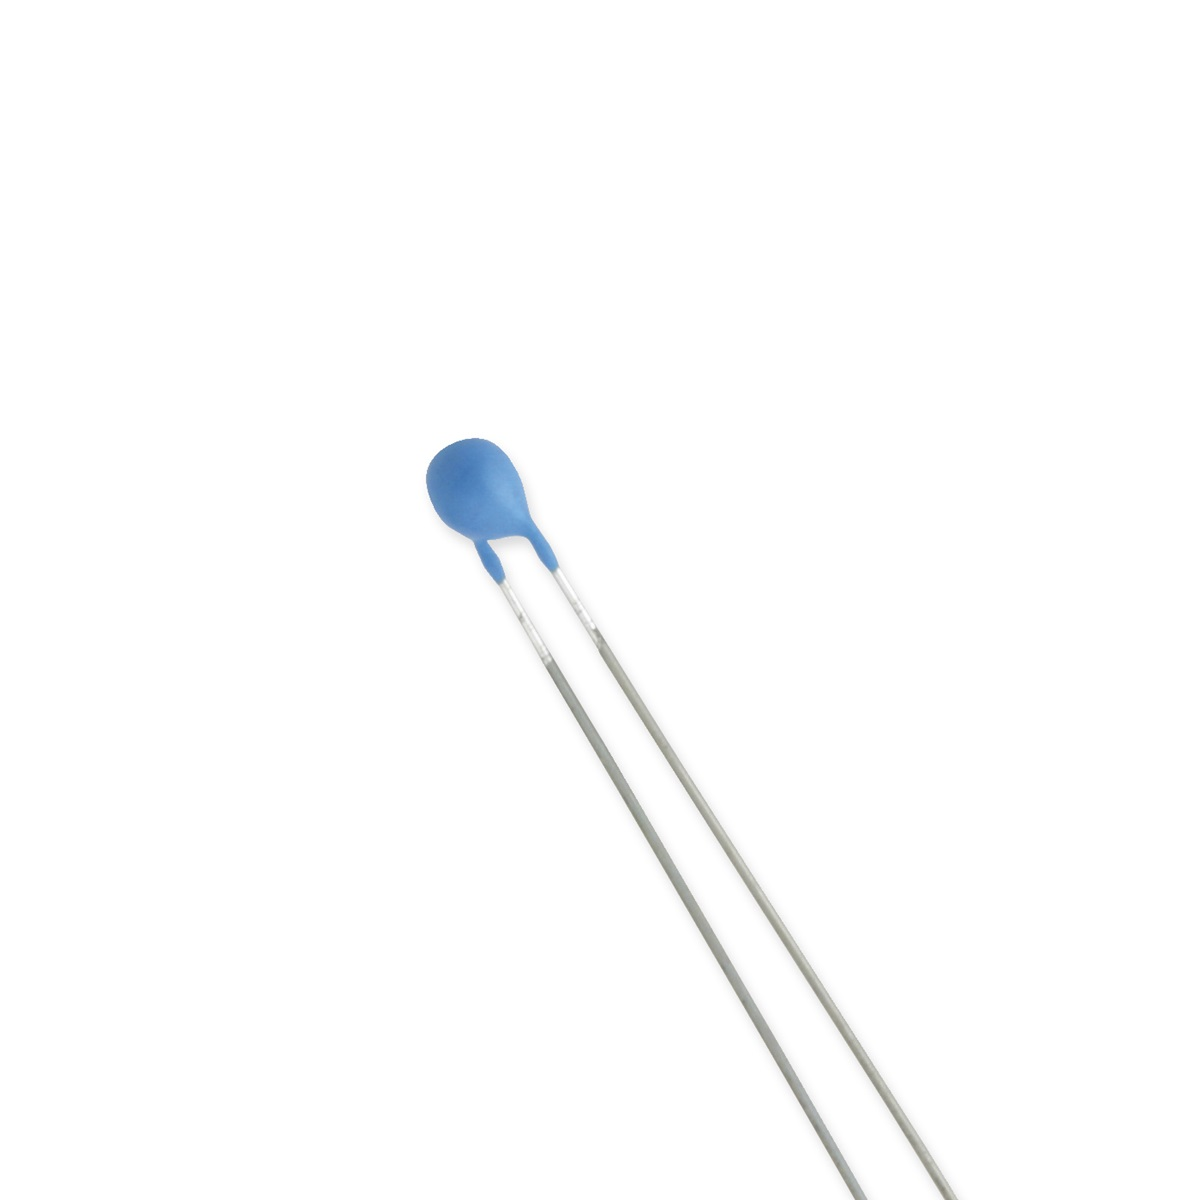
\includegraphics[width = 3cm,height=3cm]{pr303J2.jpg}};
			\begin{scope}[x={(image.south east)},y={(image.north west)}]
				\draw[color=black, ultra thin,fill=white] (0.0,0.0) rectangle (0.21,0.16) node[pos=.5] {A};
			\end{scope}
		\end{tikzpicture}
	\end{subfigure}%
	\hfill
	\begin{subfigure}[b]{0.3\textwidth}
		\begin{tikzpicture}
			\node[anchor=south west,inner sep=0] (image) at (0,0) { 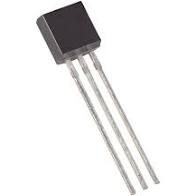
\includegraphics[width = 3cm,height=3cm]{ds18b20.jpg}};
			\begin{scope}[x={(image.south east)},y={(image.north west)}]
				\draw[color=black, ultra thin,fill=white] (0.0,0.0) rectangle (0.21,0.16) node[pos=.5] {B};
			\end{scope}
		\end{tikzpicture}
	\end{subfigure}%
	\hfill
	\begin{subfigure}[b]{0.3\textwidth}
		\begin{tikzpicture}
			\node[anchor=south west,inner sep=0] (image) at (0,0) { 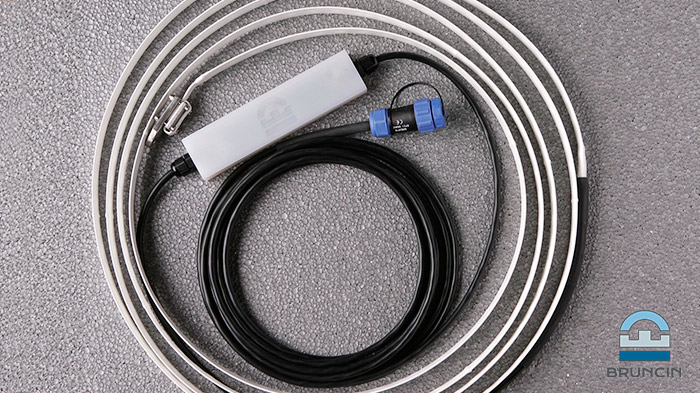
\includegraphics[width = 3cm,height=3cm]{temperature-chain-bruncin-1.jpg}};
			\begin{scope}[x={(image.south east)},y={(image.north west)}]
				\draw[color=black, ultra thin,fill=white] (0.0,0.0) rectangle (0.21,0.16) node[pos=.5] {C};
			\end{scope}
		\end{tikzpicture}
	\end{subfigure}%
	\hfill
	\caption{Examples of temperature sensors employed by remote sensing devices.These types of devices include (A) thermistors such as the PR303J2 (image source: \cite{pr303J2}), (B) digital temperature sensors such as the DS18B20 (image source: \cite{ds18b20}) and (C) digital temperature chains (DTC) such as the Bruncin DTC (image source: \cite{bruncindtc}) } 
	\label{fig:temp_examples}
\end{figure}

Temperature sensing technology is commonly used for thermal compensation as measurements such as pressure and humidity are dependent on environmental temperature \cite{mansoor2015silicon}. Thermal sensing technology exists in a variety of forms however, choice of sensor is heavily dependant on the application i.e. the object to be measured, the material state and the type of contact with the sensor \cite{mansoor2015silicon,childs2000review}. There are 3 main categories of measurement techniques \cite{childs2000review}:

\begin{enumerate}
	\item Invasive Measurements: Direct contact with an object of interest. This method is suitable for the measurement of objects in liquid or gas states. This category encompasses thermoelectric devices, liquid in glass thermometers, electronically resistive devices as well as semiconductor devices \cite{mansoor2015silicon}
	\item Semi-Invasive: Using the thermal measurement medium on an object and observing the effects of temperature such as thermal paints. Note: measurements are not directly taken from the object but rather the properties of the medium.
	\item Non-Invasive: Object is measured from a distance using a device such as an infrared camera or acoustic thermography.
\end{enumerate}

In addition, sensor selection is based on the range, accuracy, resolution and precision of the device to ensure correct use An overview of different electric sensors is given below \cite{childs2000review} A full discussion of the types of sensors is provided below where the types of technology, advantages and disadvantaeges are provided. Additionally, the technology has been selected for its implementation in the remote sensing devices shown in table \ref{tab:device_tempsense} below.
 
\begin{table}[H]
	\centering
	\caption{Comparison of the different components used by each device for temperature measurement as well as the . Each device measures temperature of a different process. For example:  the WIIB measure air temperature whereas a device like the SIMB measures temperature profiles of ice floes in addition to air temperature.}
	\label{tab:device_tempsense}
	\setlength{\extrarowheight}{5pt}
	\resizebox{\textwidth}{!}{%
	\begin{tabular}{|l|l|l|l|}
		\hline
		\textbf{Device name} & \textbf{Temperature sensor} & \textbf{Sensor type}& \textbf{Measurement Objective} \\ \hline
		WIIB & VN-100 & Digital Tempereture sensor & Air temperature \\ \hline
		WIIOS & DS18B20 & Digital temperature sensor & Air temperature \\ \hline
		NDWB & IG-500 & Digital temperature sensor &Internal ambient temperature \\ \hline
		SKIB & None & none & None \\ \hline
		SWIFT & Aquadop profiler & Thermistor & water temperature \\ \hline
		\multirow{2}{*}{SIMB} & DS18B20 & Digital temperature sensor & Air Temperature \\ \cline{2-3} 
		& Bruncin DTC & Digital temperature chain&Ice temperature profile \\ \hline
		Polar ISVP & PR303J2 & thermistor &Sea surface temperature \\ \hline
		Trident & unspecified & Not reported &Air temperature \\ \hline
	\end{tabular}
}
\end{table}

Table \ref{tab:device_tempsense} shows that the majority of devices use digital temperature sensors for ambient air temperature measurementwith thermistors begin the second temperature sensors type as used by \textcite{thomson2012wave}. Most device use temperature sensors that have been integrated into high powered IMU/AHRS systems as is the case with WIIB and NDWB. While the SWIFT buoy and the Polar ISVP both utlise the same sensing technology however the Polar ISVP used a standalone PR303J2 while the SIFT used the temperature sensor onboard the Nortek Aquadopp Profiler which is primarly a current profiler. This shows that temperature sensing was not a primary focus for this device design and this is supported by the lack of discussion regarding the performance of the temperature sensor in the literature.
\subsubsection{Thermistors}

Modern thermistors have progressed significantly in the past decade. Up until recently, they have been considered inaccurate with uncertainty ranges of up to 5\% \cite{tong2001improving}. Modern thermistors are capable of providing accuracies of up to 0.01$^\circ$. They consist of a semiconductor that changes its resistance in response to temperature \cite{childs2000review}. They have a faster response time than RTDs and work on the same principle for temperature measurement. However, where RTDs have a Positive temperature coefficient, thermistors have a negative temperature coefficient \cite{tong2001improving}. These devices can operate over a substantial, albeit relatively limited, range of $-100^\circ - 300^\circ C$. The major trade-off with these devices is the lack of standards \cite{tong2001improving}. Operating the device involves a large degree of uncertainty. Also, these devices are not powerful enough to accurately reach the desired ranges alone. They need to be coupled with similar devices. Finally, the response curve is non-linear. The  relationship between resistance and temperature is \cite{childs2000review}:
\begin{equation}
	R_T = R_0e^{1 - B(\frac{1}{T}- \frac{1}{T_0})}
\end{equation}
where $R_T$ is the temperature measured, $R_0$ is the resistance at a known temperature $T_0$, T is the temperature and B is a coefficient based on the properties of the thermistor. Finally, these devices are more prone to noise from excitation current.

\subsubsection{Silicon Temperature Devices}

Semiconductor temperature devices are suited to applications where the temperature ranges from -55 to 150 $^\circ C$ these devices are capable of providing a stable output with a typical accuracy of $0.8 ^\circ C$. These devices typically consist of diodes and transistors with a bandgap voltage that changes with a change in temperature \cite{childs2000review}. These devices are advantageous in electronic application due to their small form, high accuracy and stability. These devices are relatively simple and have a good sensitivity to changes \cite{childs2000review}. Diodes are typically used in semiconductor devices. Here, the forward voltage drop across the p-n junction is linearly proportional to the Ambient temperature over a certain temperature range (typically 25K - 400k) \cite{childs2000review}. These devices are made out of either silicon or Galium-Arsenide. Silicon is preferred as it has better stability at low temperatures and is cheaper however, this comes at the trade-off of a lower voltage output \cite{childs2000review}. \par These Types of devices are readily available in IC forms and are manufactured in a variety of packages, types and compositions for any application. Typical devices are DS18B20, LM355 or BMP2080. Recent innovations in Silicon sensing have seen the rise of CMOS devices and Micro Electrical-MEchanical Systems (MEMs) being used more frequently \cite{mansoor2015silicon}. While these devices can suffer from deterioration due to self-heating, \textcite{mansoor2015silicon} discuss that the low-power operation of these devices can offset this issue. This is advantageous for systems that are constrained by power consumption. However, a major disadvantage with these devices is that these devices work ideally with a purely DC signal.An AC coupled signal can cause significant errors in the output \cite{childs2000review} \cite{mansoor2015silicon}. These errors can be the result of improper shielding and poor grounding. Hence proper shielding and grounding are required to reduce these errors. Finally, these devices require careful calibration before use.

\subsection{Atmospheric Pressure Sensing and Sensors}

There has been an increased demand for in-situ environmental monitoring as mentioned by \cite{vichi2019effects} \cite{kennicutt2014polar} \cite{kennicutt2016delivering} \cite{kennicutt2019sustained} \cite{alberello2019drift}. It can provide insight into wind currents and storm events as well as predict trajectories of these storms. In addition, atmospheric pressure is crucial for characterizing atmospheric-ocean process such as tropical storms which create areas of low pressure during their trajectory \cite{vichi2019effects}. Current devices have employed pressure sensing techniques which have been critical for determining accurate AHRS measurements\cite{vn-100} in addition to environmental monitoring. Examples of pressure sensing devices are shown in table \ref{tab:device_press} below.

\begin{table}[H]
	\centering
	\caption{Comparison of the different pressure sensing components used by each device as well as the measurement objective guiding the selection of the component. "Not Reported" is given where a device includes a pressure sensor but provides no information to its use. "-" is given where a column does not apply to the device. "None" is given where a device does not contain a pressure sensor}
	\label{tab:device_press}
	\setlength{\extrarowheight}{5pt}
	\resizebox{\textwidth}{!}{%
		\begin{tabular}{|l|l|l|l|}
			\hline
			\textbf{Device Name} & \textbf{Pressure sensor}& \textbf{Sensor type} & \textbf{Measurement objective} \\ \hline
			WIIB & VN-100 & Digital barometric pressure sensor & Atmospheric pressure \\ \hline
			WIIOS & None &- &- \\ \hline
			NDWB & MXP-5100-AP & Piezoresistive silicon pressure sensor &Atmospheric pressure \\ \hline
			SKIB & None &- &- \\ \hline
			SWIFT & SBG Eclipse-N & Not Reported & Not Reported \\ \hline
			\multirow{2}{*}{SIMB} & \multirow{2}{*}{BME280} & \multirow{2}{*}{Digital barometric pressure sensor} & Atmospheric pressure  \\ \cline{4-4} &&& humidity\\ \hline
			Polar ISVP & PTB100 & a silicon capacitive barometric sensor & Atmospheric pressure \\ \hline
			Trident & None &- &- \\ \hline
		\end{tabular}	
}
\end{table}

While pressure is important for understanding atmospheric processes, table \ref{tab:device_press} shows that it is the least critical component for in-situ remote sensing. The WIIOS, SKIB and Trident sensors do not include a pressure sensor at all. The consequence is that these devices are not suitable for characterizing the effects of climate on sea ice as well as capturing the/predicting severe weather events such as the cyclones discussed in \textcite{vichi2019effects}. The SWIFT buoy includes the capability of pressure sensing however, do not sample the sensor for standalone pressure measurements. The devices that include pressure measurements focus on measuring atmospheric pressure through digital barometric pressure sensors \cite{rabault2019open,planck2019evolution}, piezoresistive silicon sensors \cite{doble2017robust} or silicon capacitive sensors \cite{uptempo}. Examples of these sensors are shown in figure \ref{fig:press_examples} 

\begin{figure}[H]
	\centering
	\begin{subfigure}[b]{0.3\textwidth}
		\begin{tikzpicture}
			\node[anchor=south west,inner sep=0] (image) at (0,0) { 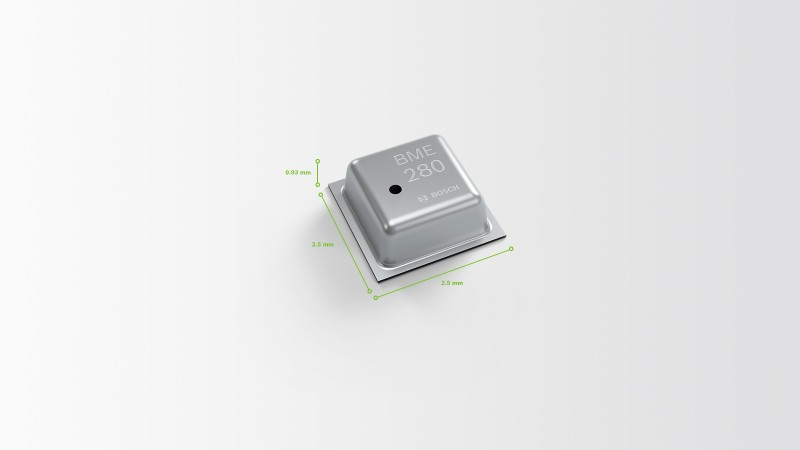
\includegraphics[width = 3cm,height=3cm]{BME280.jpg}};
			\begin{scope}[x={(image.south east)},y={(image.north west)}]
				\draw[color=black, ultra thin,fill=white] (0.0,0.0) rectangle (0.21,0.16) node[pos=.5] {A};
			\end{scope}
		\end{tikzpicture}
	\end{subfigure}%
	\hfill
	\begin{subfigure}[b]{0.3\textwidth}
		\begin{tikzpicture}
			\node[anchor=south west,inner sep=0] (image) at (0,0) { 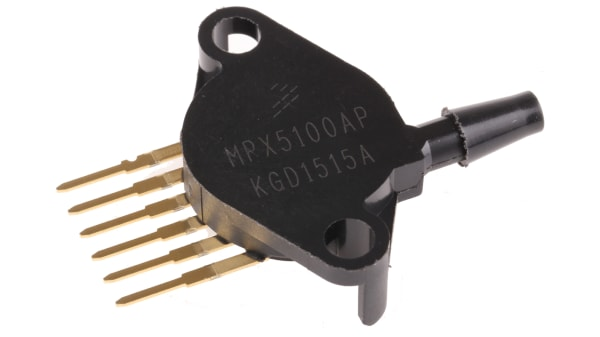
\includegraphics[width = 3cm,height=3cm]{MPX5100AP.jpg}};
			\begin{scope}[x={(image.south east)},y={(image.north west)}]
				\draw[color=black, ultra thin,fill=white] (0.0,0.0) rectangle (0.21,0.16) node[pos=.5] {B};
			\end{scope}
		\end{tikzpicture}
	\end{subfigure}%
	\hfill
	\begin{subfigure}[b]{0.3\textwidth}
		\begin{tikzpicture}
			\node[anchor=south west,inner sep=0] (image) at (0,0) { 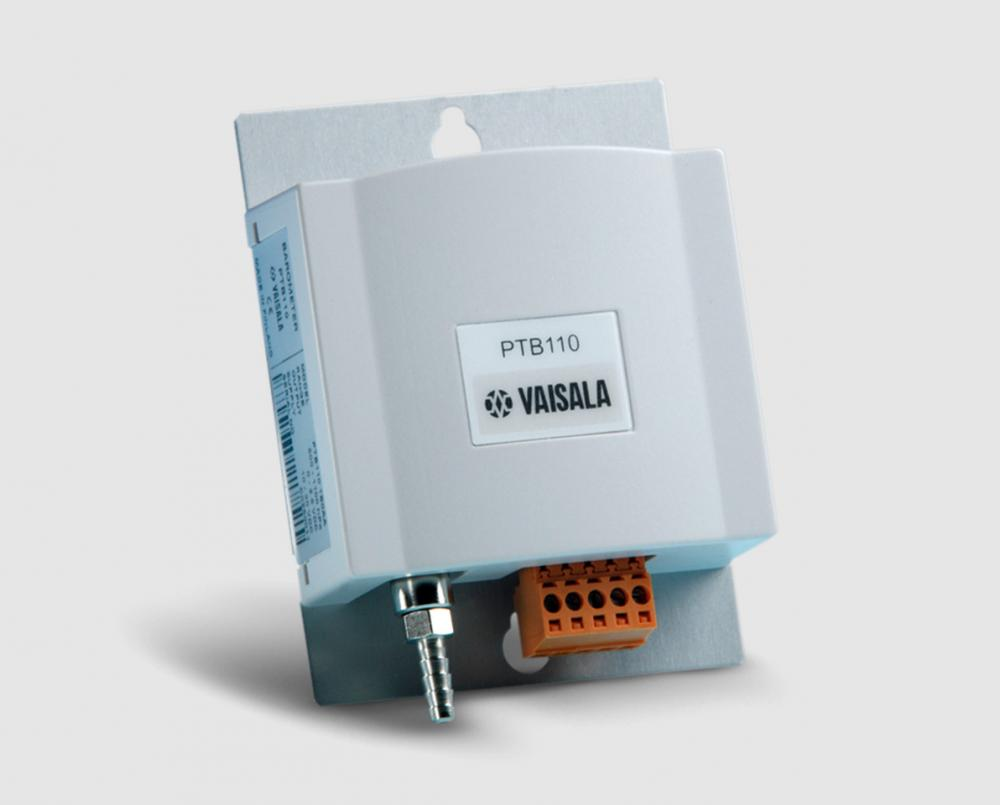
\includegraphics[width = 3cm,height=3cm]{PTB110.jpg}};
			\begin{scope}[x={(image.south east)},y={(image.north west)}]
				\draw[color=black, ultra thin,fill=white] (0.0,0.0) rectangle (0.21,0.16) node[pos=.5] {C};
			\end{scope}
		\end{tikzpicture}
	\end{subfigure}%
	\hfill
	\caption{Examples of pressure sensing technologies using a diaphragm based MEMS with different methods of measuring the strain. These are piezoresitive sensors: (A) the BME280 (image source: \cite{BME280}), (B) the MPX-5100-AP (image source: \cite{MPX5100AP}) or  capacitive sensors: (C) the PTB100 (image source: \cite{PTB110})  } 
	\label{fig:press_examples}
\end{figure}


This shows that silicon based pressure sensors are the most commonly used for remote sensing.\textcite{eaton1997micromachined} discuss the importance of micro-machined pressure sensors and provide an overview of various sensors that have been used in remote sensing devices as shown in table \ref{tab:device_press}.
\subsubsection{Diaphragm based sensors}

The current state of pressure sensing technology is driven towards Miniature MEMs version of large scale devices \cite{eaton1997micromachined}. Most large scale pressure sensors consist of a diaphragm mounted on a device in a known way. The diaphragm is coupled to a device that converts the pressure to a mechanical movement which is then measured using a gauge. These senses often had a secondary sensor that would convert the mechanical movement to an electrical signal which was then measured \cite{eaton1997micromachined} these sensors determine pressure by measuring the deflection of a miniature diaphragm. This deflection is converted to an electrical signal. Typically, a reference pressure is provided as a measurement of a sealed chamber or absolute pressure port. Assuming the simplest version of this sensor i.e. a plate of uniform thickness \cite{eaton1997micromachined} The deflection $w$ of the diaphragm is related to the pressure  $P$ by the following equation: \cite{eaton1997micromachined}

\begin{equation}
	w(r) = \frac{Pa^4}{64D}(1- (\frac{r}{a})^2)^2
\end{equation}

where r is the deformed radius of the diaphragm, a is the original radius and D is the  rigidity of the diaphragm governed by the equation:

\begin{equation}
	D = \frac{Eh^3}{12(1-v^2)}
\end{equation}
where E,h,v are Young's modulus, thickness and Poisson's ratio of the disc \cite{eaton1997micromachined}. This technique suffers from a multitude of problems namely, the diaphragm is susceptible to plastic deformation and more robust diaphragms result in more complex relationships. The current relationship is nonlinear and can result in calculation errors. Eaten (1997) advocate for the use of MEMs based electronics on these principles.

\subsubsection{Piezoresistive Sensors}

Piezoresistive sensors are electric devices constructed out of a semiconductor whose electrical properties change when a stress is applied \cite{eaton1997micromachined}. these devices are mounted to a diaphragm and exhibit a linear change in resistance with a change in Pressure. Currently, these sensors take the form of single-crystal diaphragms with piezoelectric resistors diffused through the materials. The advantage of these devices is robustness towards hysteresis and measurement drift. At low temperatures, silicon exhibits near-perfect elastic behaviour and is  3 times the tensile strength of strain gauges\cite{eaton1997micromachined}. The sensors are, however susceptible to thermal expansion and can exhibit significant temperature drift \cite{samaun1971ic}. Additionally, these sensors require resistors with identical temperature Resistance characteristics otherwise the measurements will be inaccurate. Finally, additional compensation techniques are required.

\subsubsection{capacitive sensors}

These sensors consist of parallel conductive plates. Assuming a constant, known dielectric, an external pressure causes the plates to deform which changes the capacitance C according to the relationship \cite{eaton1997micromachined}
\begin{equation}
	C = \int \int \frac{\epsilon}{d - w(r)}drd\theta
\end{equation}

where $w(r)$ is the deformation of the plate, $\epsilon$ is the strain experienced on the plate and d is the distance of separation. The Pressure capacitance relationship can be approximated using a least-squares fit \cite{eaton1997micromachined} however this results in model errors of 1.5\% and up to 11\% at $w = \frac{1}{2}h$ the height of the plate. These sensors are more advantageous over piezoresistive sensors as they have higher pressure sensitivity and reduced susceptibility to temperature drift. However, these sensors are significantly susceptible to parasitic capacitance which can result in losses and errors. Additionally, these sensors are simple in design however they tend towards more complex circuit requirements.

 
\section{Conclusion}

From the system analysis, we can see that all devices were successful in communicating remotely with a user through the Iridium satelite network due to its high area coverage and reliability. However, due to network and bandwidth constraints, most devices compensated for this by implementing computationally intensive algorithms to compress data into the required bandwidth, the popular choice for network modems is the 9603 which is ideal for its low power consumption, small form factor and relatively low cost however it only allows for short burst data transmissions. For continuous transmissions, the 9523 modem is ideal \par 

Systems were able to operate remotely for long periods of time using batteries as a power source. Lithium batteries and Alkaline batteries were the most prevalent as primary power sources allowing devices such as the WIIOS to survive for a maximum of 39 days. \textcite{doble2017robust} showed that in the Arctic marginal ice zone by coupling a solar power to a secondary lead acid battery, the device could survive for up to a year without human intervention however, \textcite{rabault2020development} achieved lower surviviabilty even with an onboard solar panel. Additional energy harvesting techniques are required in order for secondary power source to be viable. \par 

In spite of advances in power optimization, the marginal ice zone is a dangerous region. A significant number of devices were reported by \textcite{doble2017robust} to have failed when devices were frozen over and failed to recover during sea ice melt. Additionally, polar storms and large swells caused the WIIOS buoys to offline during their deployments \textcite{kohout2015device,alberello2019drift}. Additional sources of failiure have been attributed to freezing over \textcite{rabault2018investigation} however, this was due to the device being placed in the ground allowing it to be covered by snow growth \cite{barber2005microwave} and flooding. Additionally, \textcite{rabault2019open} reported failures due to rafting and ridging of ice floes which critically damaged devices.\par 

From the system analysis, we can determine that the most important measurement objectives are:
\begin{itemize}
	\item Ice drift
	\item Wave in ice measurements
	\item Ambient temperature
	\item Atmospheric pressure
\end{itemize}

Wave analysis is the most computationally expensive measurement objective as 
table \ref{tab:device_imumeasure} show that raw imu time series measured by each wave sensing device was sampled above 2Hz \cite{kohout2015device}. Advanced filtering techniques were required to compensate for the effects of low drift and biases. Some devices achieved this by using components with integrated filters such as the VN-100 AHRS sensor however, these components  are expensive and resulted in a higher overall cost for the device \cite{guimaraes2018surface}. Additionally, devices such as WIIOS and SWIFT required more expensive, more power processors to compensate for higher data rates and advanced processing algorithms. \par 

Additionally, all devices used a GPS to measure sea ice drift showing that these devices are reliable enough to perform these measurements \cite{doble2017robust}. A sample time of atleast 3 hours between GPS measurements is required to accurately capture sea ice dynamics such as oscillations and collisions. \textcite{thomson2012wave} additionally show that GPS velocity measurements are suitable for wave measurements in addition to telemetry and used these measurements to determine the orbital motion of waves. However, the positional accuracy of GPS is not suitable for measuring significant wave height as the uncertainty in positional measurements is too high ($\pm$ 5 m). GPS readings are affected by Ionospheric interference which causes a phase delay resulting in a dilation of precision (DOP), this can also be caused by the spread of satellites, azimuth and number of satellites used to take measurements. Hence, these measurements form a critical part for statistical analysis of GPS signals as this section was under-reported in the current literature. \par 

Finally, environmental sensing is critical to determining the conditions around sea ice formation. Temperature and pressure changes are key indicators of short term weather events such as polar cyclones and as such, All devices employ some form of temperature measurement either actively through components such as thermistors, and silicon temperature devices or passively embedded in higher powered sensors such as an AHRS. Additionally, the effects of temperature sensing on atmospheric temperature measurements were significantly under-reported in the literature as was the effect of pressure sensing.  Pressure sensing was also the least critical objective for the devices as this device was excluded from three out of eight devices while the SWIFT buoy had pressure sensing capabilities, this feature was not used. Hence, more research is required to fill in this knowledge gap to understand the effects of environmental sampling and their impact on climate measurements. \par

In conclusion, while the literature shows breakthroughs in low cost in situ remote sensing in the marginal ice zone, some of the effects remain unknown. Devices are still extremely specialised however, open-source, off the shelf devices can pave the way for more accessible, more affordable devices thereby increasing access to science and increasing our understanding of the marginal ice zone.